\chapter{Configurazione dell'MQTT Binding per un sistema IOT}
Per testare openHAB con un sistema IOT si \'e deciso di procedere allo sviluppo di uno {\em Smart Garden}, ovvero un sistema per la gestione automatizzata del proprio giardino. Di base si tratta di un sensore per la misurazione dell'umidit\'a del terreno e una pompa per l'attivazione dell'innaffiamento in caso di siccit\'a.

\section{Smart Garden}
Il sistema IOT quindi nello specifico \'e composto da:
\begin{itemize}
    \item \textbf{Soil Moisture Sensor}: sensore di umidit\'a del terreno (Figura \ref{fig:soil_moisture_sensore}).
    \item \textbf{Water Pump}: pompa dell'acqua utile per irrigare alla sua attivazione (Figura \ref{fig:water_pump}).
    \item \textbf{Raspberry Pi}: unit\'a logica che permette di rendere dinamica l'interazione tra i sensori. \'E la centralina del sistema IOT (Figura \ref{fig:raspberry_pi}).
    \item \textbf{Rel\'e}: elemento utile per l'attivazione e disattivazione della pompa (Figura \ref{fig:rele}).
    \item \textbf{Alimentatore da 12 Volt}: alimentazione della pompa (Figura \ref{fig:12v_power_supply}).
\end{itemize}

\subsubsection{Soil Moisture Sensore}
\begin{figure}
    \centering
    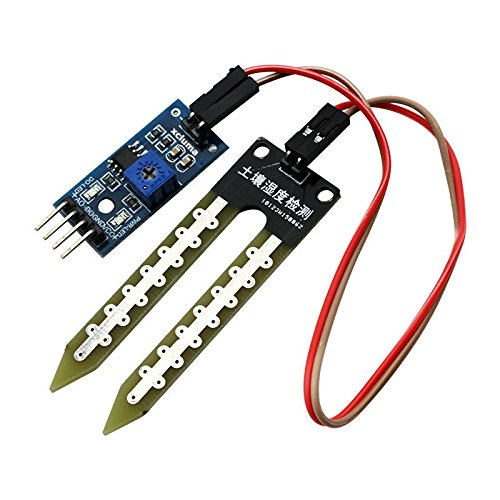
\includegraphics[width=8cm]{Immagini/soil_moisture_sensore}
    \caption{Soil Moisture Sensore}
    \label{fig:soil_moisture_sensore}
\end{figure}
Il {\em Soil Moisture Sensor} \'e un sensore che rileva l'umidit\'a del suolo. Esso ha una forma a ferro di cavallo dove alle due estremit\'a vi sono due contatti. Tra i contatti del sensore viene fatta passare una tensione, tanto maggiore è l'umidit\'a tra i due contatti, tanto minore sar\'a la resistenza, permettendo alla corrente di fluire da un contatto verso l'altro. 

Esso ha lo scopo di segnalare o meno la presenza di umidit\'a cos\'i da scatenare poi l'evento di start o stop della pompa dell'acqua. Il sensore viene collegato per mezzo di cavi ai pin della Raspberry Pi per inviare segnali di input.

\subsubsection{Water Pump}
\begin{figure}
    \centering
    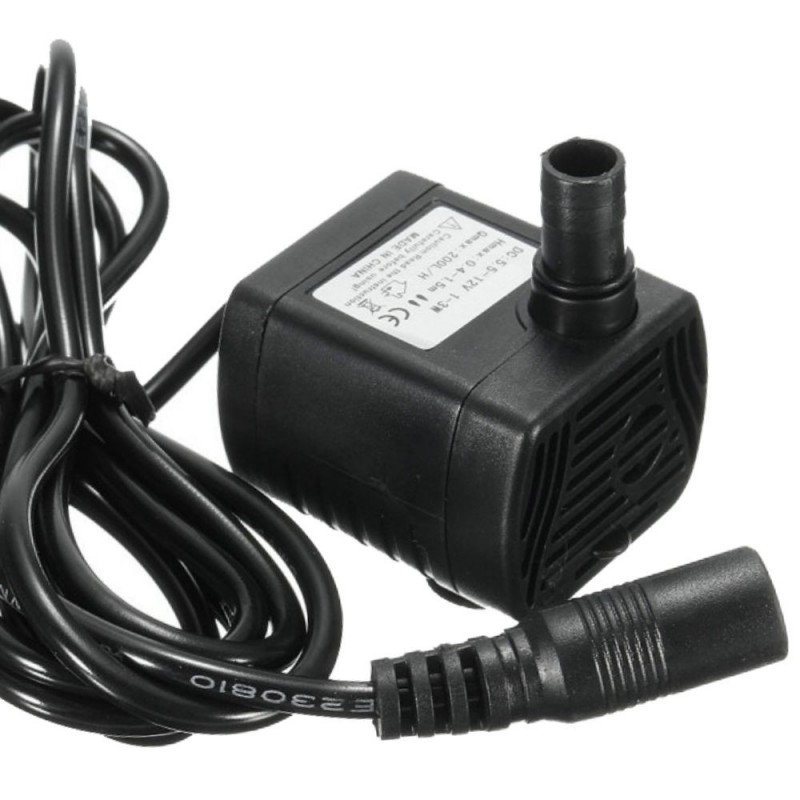
\includegraphics[width=8cm]{Immagini/water_pump}
    \caption{Water Pump}
    \label{fig:water_pump}
\end{figure}
La Pompe dell'Acqua permette di prendere l'acqua e dirigerla verso una direzione per l'irrigazione del proprio giardino. Essa ha la caratteristica di essere totalmente immersa nell'acqua e presenta nella parte superiore un buco nella quale viene infilato un tubo che sar\'a poi collegato nell'altra estremit\'a ad un erogatore d'acqua utile ad innaffiare.

La Pompa viene collegata tramite cavi ad un Rel\'e per la sua attivazione ed all'alimentatore da 12 volt poiché la raspberry non pu\'o sostenere tale carico. Essa viene attivata in caso di siccit\'a e spenta altrimenti.

\subsubsection{Raspberry Pi}
\begin{figure}
    \centering
    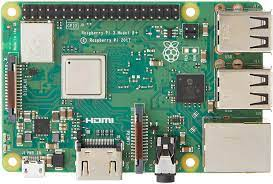
\includegraphics[width=8cm]{Immagini/raspberry_pi}
    \caption{Raspberry Pi}
    \label{fig:raspberry_pi}
\end{figure}
Centralina del sistema IOT. Essa permette di essere programmata per leggere e controllare i vari dispositivi che gli vengono collegati. Per collegarsi ad un sessore o dispositivo esterno vengono messsi a disposizione dei pin ai quali vengono agganciati dei cavi.

La Raspberry viene collegata ai vari sensori e dispositivi per implementare la logica del sistema.

La Raspberry Pi \'e dotata di una scheda di rete tramite la quale comunicher\'a esternamente con il device in cui \'e installato openHAB.

\subsubsection{Rel\'e}
\begin{figure}
    \centering
    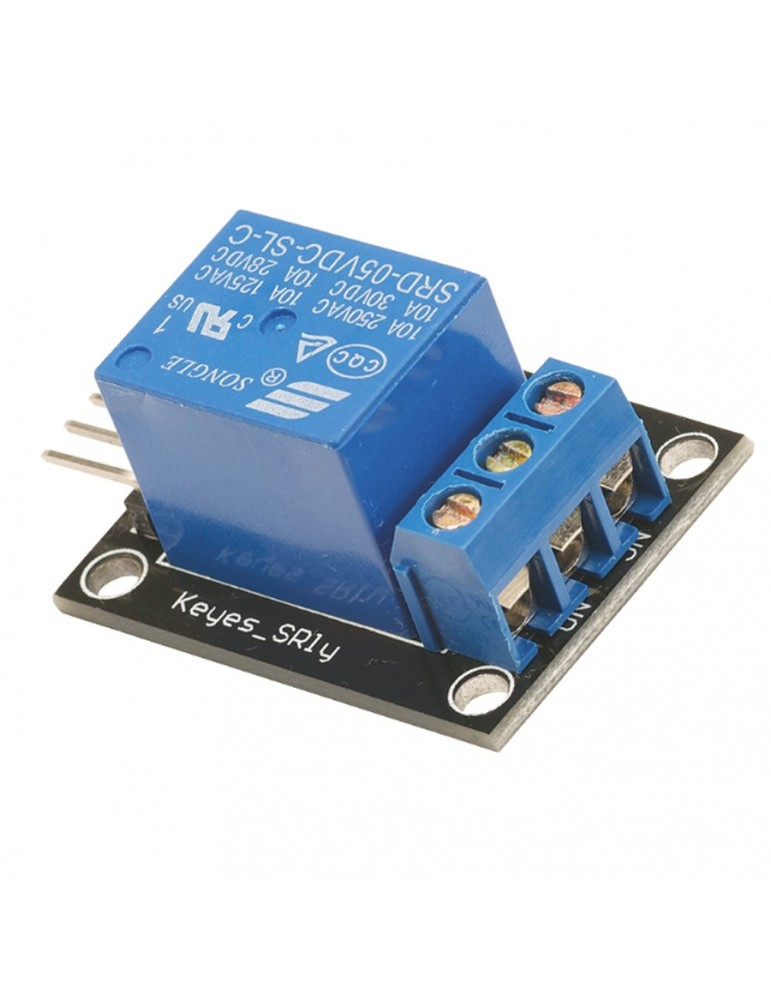
\includegraphics[width=8cm]{Immagini/rele}
    \caption{Rel\'e}
    \label{fig:rele}
\end{figure}
Elemento che permette tramite il passaggio della corrente di attivarsi o disattivarsi. Esso \'e come un pulsante che si accende e si spegne al passaggio della corrente.

Utile nel sistema per attivare e disattivare la Pompa. La Raspberry quando vuole attivare/disattivare la Water Pump attiva/disattiva il Rel\'e che a sua volta attiva/disattiva il circuito tra Pompa e la sua alimentazione.

\subsubsection{Alimentatore da 12 Volt}
\begin{figure}
    \centering
    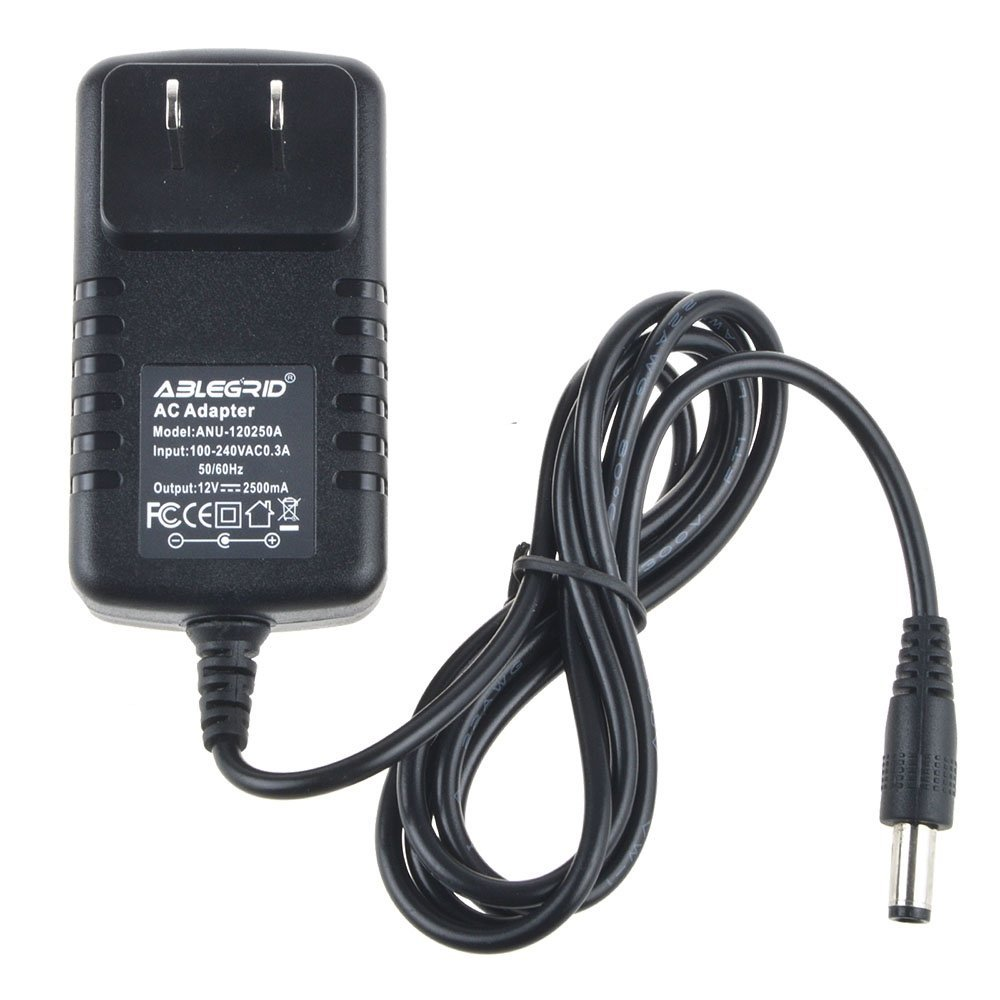
\includegraphics[width=8cm]{Immagini/12v_power_supply}
    \caption{Alimentatore da 12 Volt}
    \label{fig:12v_power_supply}
\end{figure}
Alimentazione utile per attivare la pompa. Essa non poteva funzionare con l'alimentazione fornita da Raspberry che arriva massimo a 5 volt. 

L'alimentatore viene collegato al Rel\'e e alla pompa.

\'E possibile visualizzare un semplice schema dei collegamenti a Figura \ref{fig:smart_garden_structure}.

\begin{figure}
    \centering
    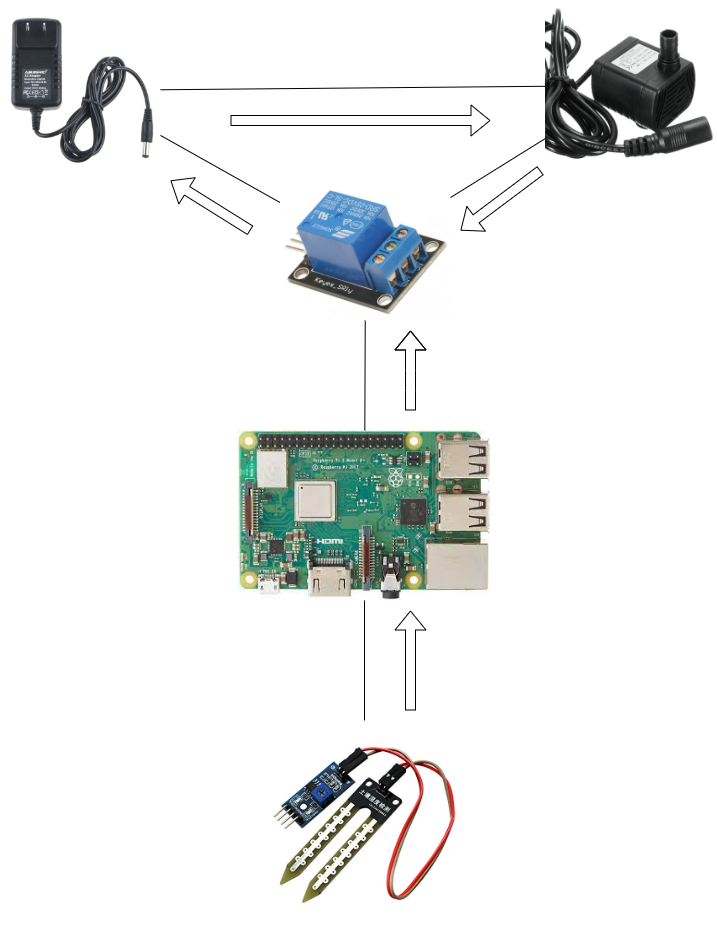
\includegraphics[width=12cm]{Immagini/smart_garden_structure}
    \caption{Struttura Smart Garden}
    \label{fig:smart_garden_structure}
\end{figure}

\subsection{Sviluppo sistema IOT}
Il sistema IOT viene controllato tramite Raspberry Pi da un piccolo programma python. Esso ha accesso tramite la libreria \texttt{RPi.GPIO} ai pin per gestire i dispositivi o sensori agganciati. Il programma legge in input il valore prelevato dal sensore di umidit\'a mentre attiva e disattiva in output la pompa tramite il rel\'e. Tutto ci\'o viene gestito tramite protocollo MQTT con libreria \texttt{paho.mqtt.client}. Tramite dei topic infatti si pu\'o:
\begin{itemize}
    \item leggere il sensore di umidit\'a
    \item attivare o disattivare la pompa manualmente
    \item attivare o disattivare il sistema in modalit\'a automatica, ovvero sar\'a lui ad attivare o disattivare la pompa in caso non ci sia o ci sia un terreno umido.
\end{itemize}

\subsubsection{Codice del sistema IOT}
Il programma \'e composto da 4 file principali.
\begin{itemize}
    \item \textbf{Soil.py}: contiene la classe per la creazione dell'oggetto capace di gestire il sensore di umidit\'a del terreno.
    \item \textbf{Pump.py}: contiene la classe per la creazione dell'oggetto capace di gestire il rel\'e per controllare la pompa dell'acqua.
    \item \textbf{MQTTClient.py}: contiene la classe per la creazione dell'oggetto capace di fare publish e subscribe in MQTT.
    \item \textbf{main.py}: file main da cui ha inizio il programma ed in cui \'e la logica di business.
\end{itemize}

\begin{lstlisting}[caption=Soil.py, label=code:soil.py]
import RPi.GPIO as GPIO

class Soil:

    def __init__(self, channel):
        self.channel = channel
        GPIO.setmode(GPIO.BCM)
        GPIO.setup(self.channel, GPIO.IN)

    def status(self):
        return GPIO.input(self.channel)
\end{lstlisting}

\begin{lstlisting}[caption=Pump.py, label=code:pump.py]
import RPi.GPIO as GPIO

class Pump:

    def __init__(self, channel):
        self.channel = channel
        GPIO.setmode(GPIO.BCM)
        GPIO.setup(self.channel, GPIO.OUT)

    def on(self):
        GPIO.output(self.channel, GPIO.HIGH)

    def off(self):
        GPIO.output(self.channel, GPIO.LOW)
\end{lstlisting}

\begin{lstlisting}[caption=MQTTClient.py, label=code:mqtt_client.py]
import paho.mqtt.client as mqtt

class MQTTClient:

    def __init__(self, ip, port):
        self.ip = ip
        self.port = port

    def publish(self, topic, to_publish):
        self.client = mqtt.Client()
        self.client.connect(self.ip, self.port, 60)
        self.client.publish(topic, to_publish, 0, True);
        self.client.disconnect()

    def subscribe(self, topic, on_message):
        client = mqtt.Client()
        client.connect(self.ip, self.port, 60)
        client.on_connect = lambda client, userdata, flags, rc : self.on_connect(client, userdata, flags, rc, topic)
        client.on_message = on_message
        client.loop_start()
        return client

    def on_connect(self, client, userdata, flags, rc, topic):
        print("[" + topic + "]: connected with result code " + str(rc))
        client.subscribe(topic)
\end{lstlisting}

\begin{lstlisting}[caption=main.py, label=code:main.py]
import time
import threading

from MQTTClient import MQTTClient
from Soil import Soil
from Pump import Pump

import os
from os.path import join, dirname
from dotenv import load_dotenv

dotenv_path = join(dirname(__file__), '.env')
load_dotenv(dotenv_path)

# mqtt connection data
MQTT_IP = os.environ.get("MQTT_IP")
MQTT_PORT = (int)(os.environ.get("MQTT_PORT"))

# topics
TOPIC_HANDLE_PUMP = os.environ.get("TOPIC_HANDLE_PUMP")
TOPIC_HANDLE_AUTO = os.environ.get("TOPIC_HANDLE_AUTO")
TOPIC_STATUS_SOIL = os.environ.get("TOPIC_STATUS_SOIL")

# pins
PIN_PUMP = (int)(os.environ.get("PIN_PUMP"))
PIN_SOIL = (int)(os.environ.get("PIN_SOIL"))

# global variable to start and stop auto
stop_thread = True

mqtt_client = MQTTClient(MQTT_IP, MQTT_PORT)

soil = Soil(PIN_SOIL)
pump = Pump(PIN_PUMP)

# threading functions
def publish_pump(status):
    global status_thread
    if not stop_thread:
        mqtt_client.publish(TOPIC_HANDLE_PUMP, status)

def callback():
    if soil.status():
        publish_pump('ON')
        mqtt_client.publish(TOPIC_STATUS_SOIL, 'Water Not Detected')
    else:
        publish_pump('OFF')
        mqtt_client.publish(TOPIC_STATUS_SOIL, 'Water Detected')

def loop():
    while True:
        callback()
        time.sleep(1)

# on_message functions
def on_message_auto(client, userdata, msg):
    global stop_thread
    stop_thread = msg.payload.decode() != "ON"

def on_message_pump(client, userdata, msg):
    global pump
    if msg.payload.decode() == "ON":
        pump.on()
    else:
        pump.off()

# main function
if __name__ == "__main__":
    thread = threading.Thread(target=loop)
    thread.start()
    mqtt_client.subscribe(TOPIC_HANDLE_AUTO, on_message_auto)
    mqtt_client.subscribe(TOPIC_HANDLE_PUMP, on_message_pump)
\end{lstlisting}

In breve alla partenza del programma vengono inizializzate le costanti prelevate dalle variabili d'ambiente relative a 
\begin{itemize}
    \item \textbf{MQTT\_IP}: IP del client MQTT.
    \item \textbf{MQTT\_PORT}: porta del client MQTT.
    \item \textbf{TOPIC\_HANDLER\_PUMP}: topic MQTT per gestire l'attivazione e la disattivazione manuale della pompa.
    \item \textbf{TOPIC\_HANDLER\_AUTO}: topic MQTT per gestire l'attivazione e la disattivazione della modalit\'a automatica.
    \item \textbf{TOPIC\_STATUS\_SOIL}: topic MQTT per leggere lo stato del sensore di umidit\'a del suolo.
    \item \textbf{PIN\_PUMP}: pin di controllo della pompa.
    \item \textbf{PIN\_SOIL}: pin per la lettura del valore dal sensore di umidit\'a.
\end{itemize}

Poi vengono inizializzati i vari oggetti relativi alla gestione sia dei sensori che del client MQTT. Oltre a questi viene inizializzato un flag chiamato \texttt{stop\_thread} utile ad avviare e fermare l'esecuzione della modalit\'a automatica.

\paragraph{Modalit\'a automatica}
Successivamente viene riportato lo sviluppo della modalit\'a automatica, ovvero l'esecuzione di un thread che permette di mettere in un loop infinito una funzione capace di prelevare il dato dal sensore di umidit\'a e attivare o disattivare la pompa in caso di siccit\'a o presenza di acqua. Il loop aspetta sempre un intervallo di un secondo. Inoltre la funzione viene eseguita solamento se la variabile globale \texttt{stop\_thread} \'e False. 

In realt\'a quindi l'esecuzione del thread serve per prelevare il dato in input dal sensore di umidit\'a e solo se il flag rispetta la condizione viene attivata o disattivata la pompa; quindi l'esecuzione automatica avviene per mezzo dell'attivazione del flag.

Oltre ad essere letti, i dati vengono anche notificati tramite un publish MQTT; ovvero vengono notificati sia i cambiamenti di stato del sensore di umidit\'a, sia l'accenzione o spegnimento della pompa al topic della modalit\'a manuale.

\paragraph{Esecuzione}
All'esecuzione del programma quindi viene fatto partire il thread per prelevare il dato dal sensore di umidit\'a con il flag per la modalit\'a automatica disabilitato, dopodich\'e vengono inizializzati i subscriber MQTT per l'attivazione della pompa in modalit\'a manuale e automatica.

\subsection{Broker MQTT}
Come {\em Broker MQTT} si \'e pensato di usare un software open source come \textbf{Mosquitto}. Esso pu\'o essere scaricato tranquillamente su macchina linux tramite il comando 

\texttt{sudo apt install mosquitto}

e si attiva subito. Esso viene attivato in automatico ogni volta che si riavvia la macchina che lo ospita.

Ai client MQTT che gli si collegano basta dargli indirizzo IP e la porta (1883 di default). Esso pu\'o essere installato in qualsiasi dispositivo interno alla rete. Nel caso specifico di questa sperimentazione \'e stato installato per comodit\'a nella Raspberry Pi dello {\em Smart Garden}.

\subsection{MQTT Binding del sistema IOT}
OpenHAB e lo {\em Smart Garden} quindi comunicano tramite protocollo MQTT.

In una prima fase \'e stato implementato uno sviluppo tramite protocollo REST ma dopo alcuni test \'e risultato essere molto pesante e inadatto per un sistema come questo. Esso infatti, non essendo di tipo publish/subscribe, obbligava openHAB a fare delle chiamate in loop per prelevare i dati. Tale approccio appesantisce di molto la rete nel caso le chiamate vengano fatte molto di frequente mentre nel caso contrario non garantisce un'esperienza real time.

Al contrario con MQTT entrambi i client (openHAB e lo Smart Garden) si sottoscrivono ai topic e notificano tramite questi i vari cambiamenti.
I topic sono:
\begin{itemize}
    \item \textbf{handle/pump}: per abilitare (inviando il messaggio ``\textbf{ON}'') o disabilitare (inviando il messaggio ``\textbf{OFF}'') la pompa dell'acqua manualmente.
    \item \textbf{handle/auto}: per abilitare (inviando il messaggio ``\textbf{ON}'') o disabilitare (inviando il messaggio ``\textbf{OFF}'') la modalit\'a di innaffiamento automatica. In tal caso, come visto precedentemente tale attivazione scatena da parte dello {\em Smart Garden} una pubblicazione del topic {\em handle/pump} una mutazione nel caso venga attivata o no la pompa dell'acqua.
    \item \textbf{status/soil}: per visualizzare i cambiamenti di stato del sensore di umidit\'a del terreno. Nel caso rileva umidit\'a verr\'a inviata dal publisher la stringa ``\textbf{Water detected}'', mentre ``\textbf{Water not detected}'' altrimenti''.
\end{itemize}

I client quindi comunicano tra loro per mezzo del broker MQTT {\em Mosquitto} installato sulla Raspberry Pi del sistema IOT. I messaggi che vengono inviati da entrambi le parti sono {\em retained}, cos\'i da mantenere l'ultimo stato inviato.

\section{Configurazione openHAB}
Dopo aver installato il framework tramite il sito ufficiale i primi passaggi per configurarlo sono:
\begin{enumerate}
    \item far partire il programma tramite l'eseguibile relativo al sistema operativo utilizzato (windows: \texttt{start.bat}, linux/mac: \texttt{start.sh})
    \item accedere alla ui web tramite l'url \texttt{http://localhost:8080/}
    \item creare l'account amministratore inserendo nome utente e password e premendo su ``Crea Account'' (Figura \ref{fig:create_admin})
    \begin{figure}
        \centering
        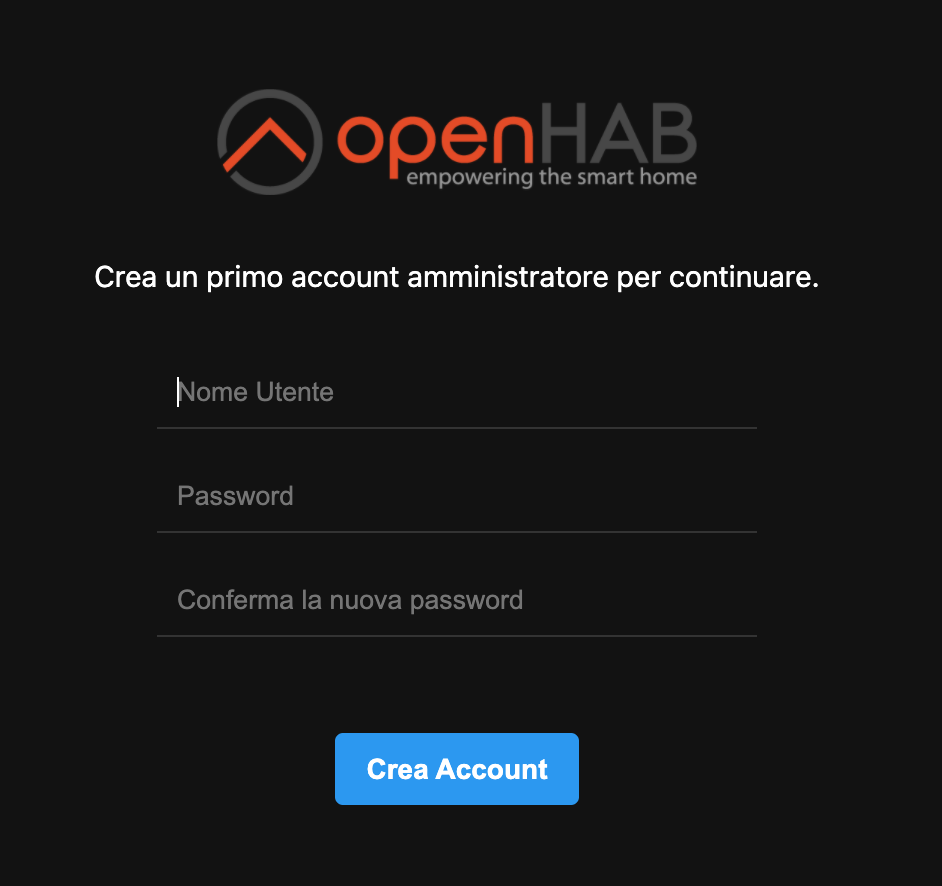
\includegraphics[width=12cm]{Immagini/create_admin}
        \caption{Crea Utente Amministratore}
        \label{fig:create_admin}
    \end{figure}
    \item impostare lingua regione e fuso orario e premere su ``Inizia Installazione'' (Figura \ref{fig:language_region}
    \begin{figure}
        \centering
        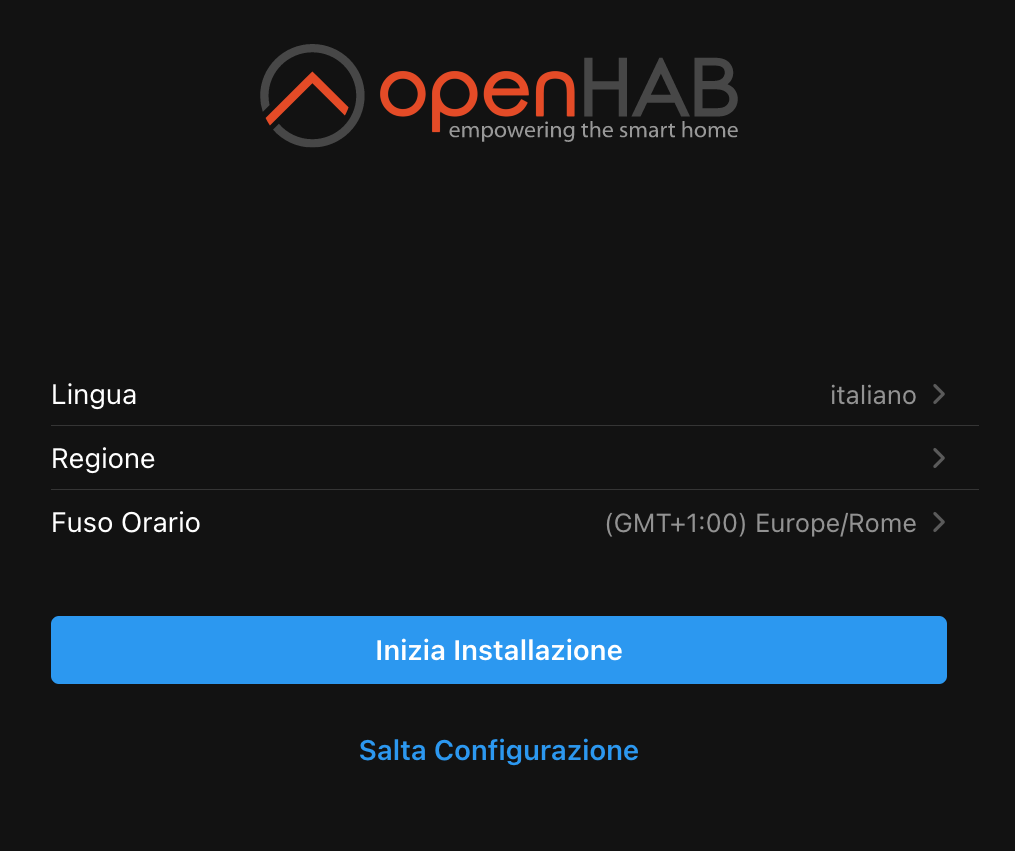
\includegraphics[width=12cm]{Immagini/language_region}
        \caption{Impostazione Lingua Regione e Fuso orario}
        \label{fig:language_region}
    \end{figure}
    \item impostare la posizione (Figura \ref{fig:location})
    \begin{figure}
        \centering
        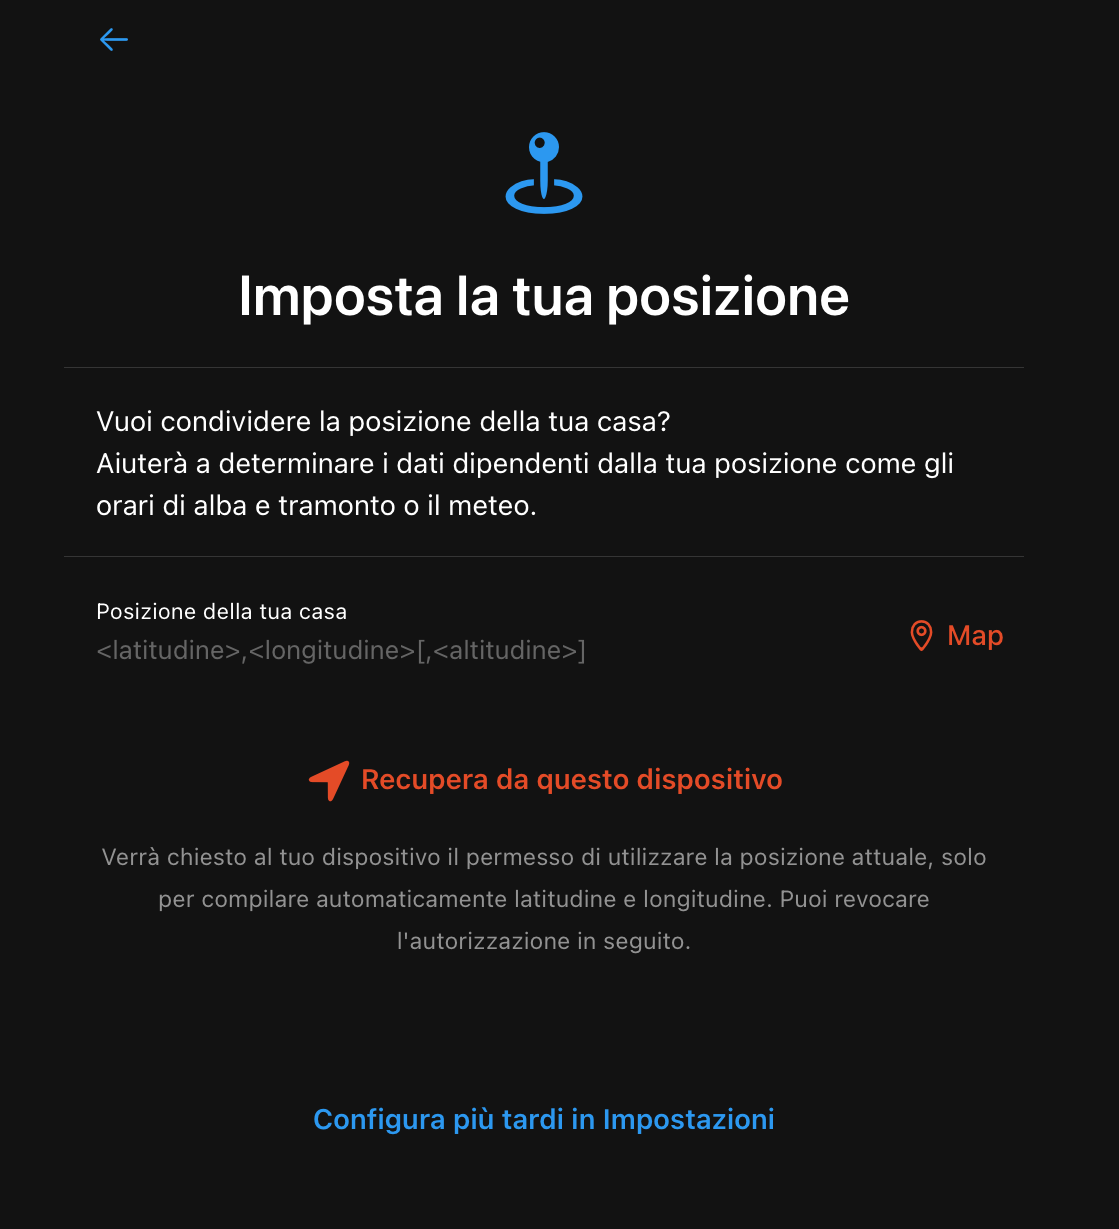
\includegraphics[width=12cm]{Immagini/location}
        \caption{Impostazione Posizione}
        \label{fig:location}
    \end{figure}
    \item installare Add-on, in questo caso \'e stato selezionato il binding MQTT. Per fare ci\'o basta premere la scritta ``Seleziona gli add-on da installare'' e selezionare \textbf{MQTT Binding}. Finita tale procedura premere su ``Installa 1 add-on'' per continuare (Figura \ref{fig:add_on})
    \begin{figure}
        \centering
        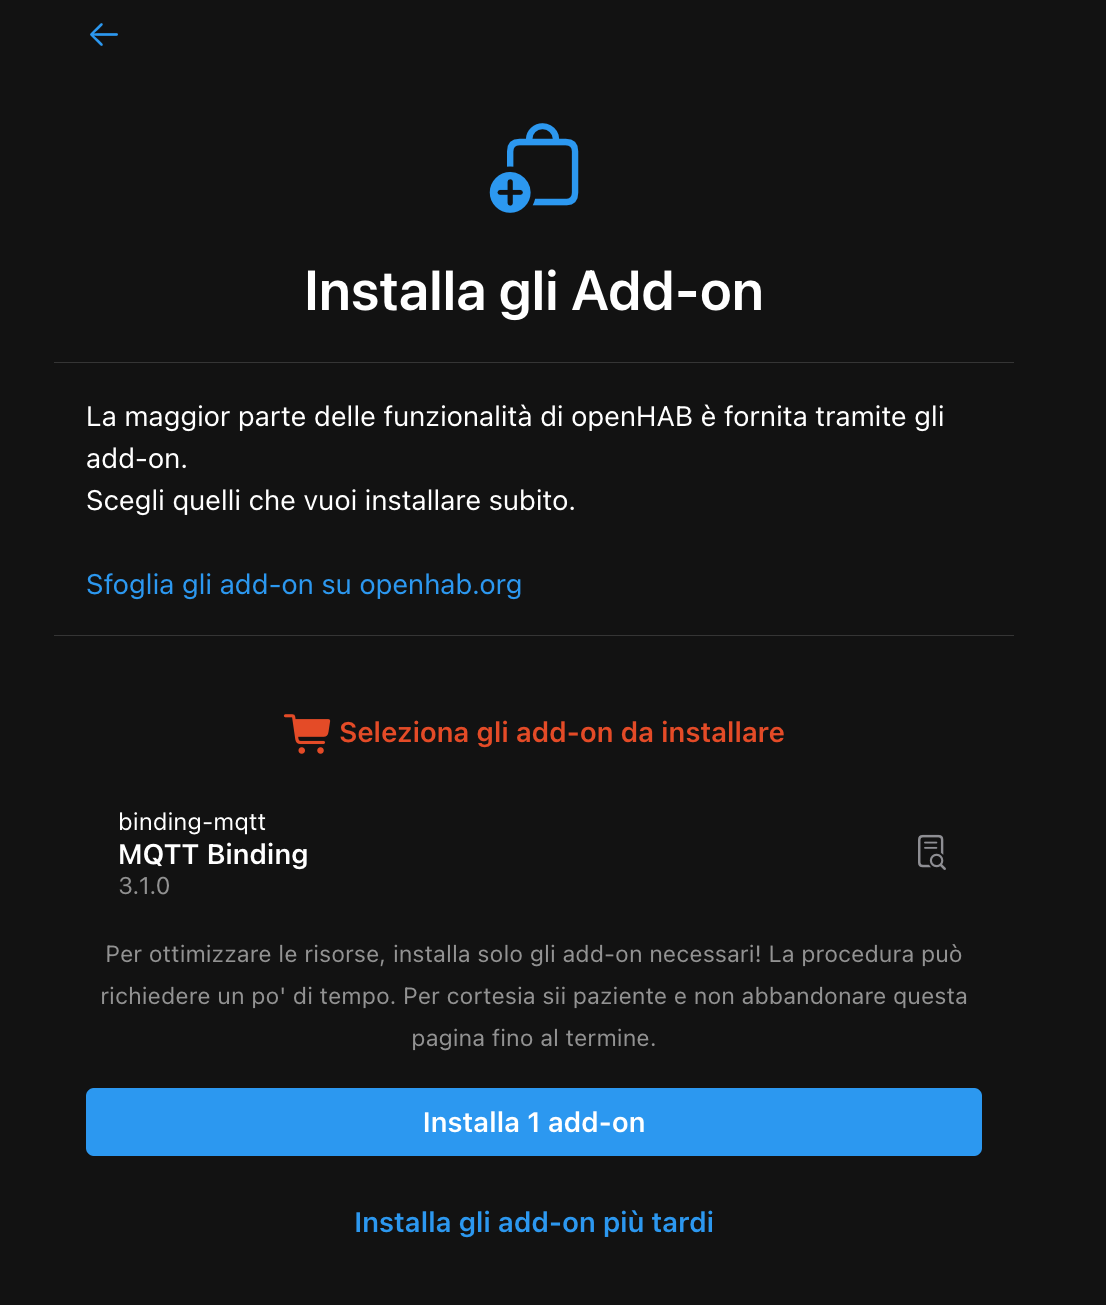
\includegraphics[width=12cm]{Immagini/add_on}
        \caption{Selezionare Add-ons}
        \label{fig:add_on}
    \end{figure}
    \item premere su ``Cominciamo''
\end{enumerate}

\subsection{MQTT Binding di openHAB}
Eseguita la configurazione iniziale ora passiamo a configurare il Binding MQTT per collegare openHAB allo Smart Garden. I passaggi sono i seguenti:
\begin{enumerate}
    \item dalla schermata principale premere su ``Impostazioni'' e successivamente su ``Things'' (Figura \ref{fig:schermata_impostazioni})
    \begin{figure}
        \centering
        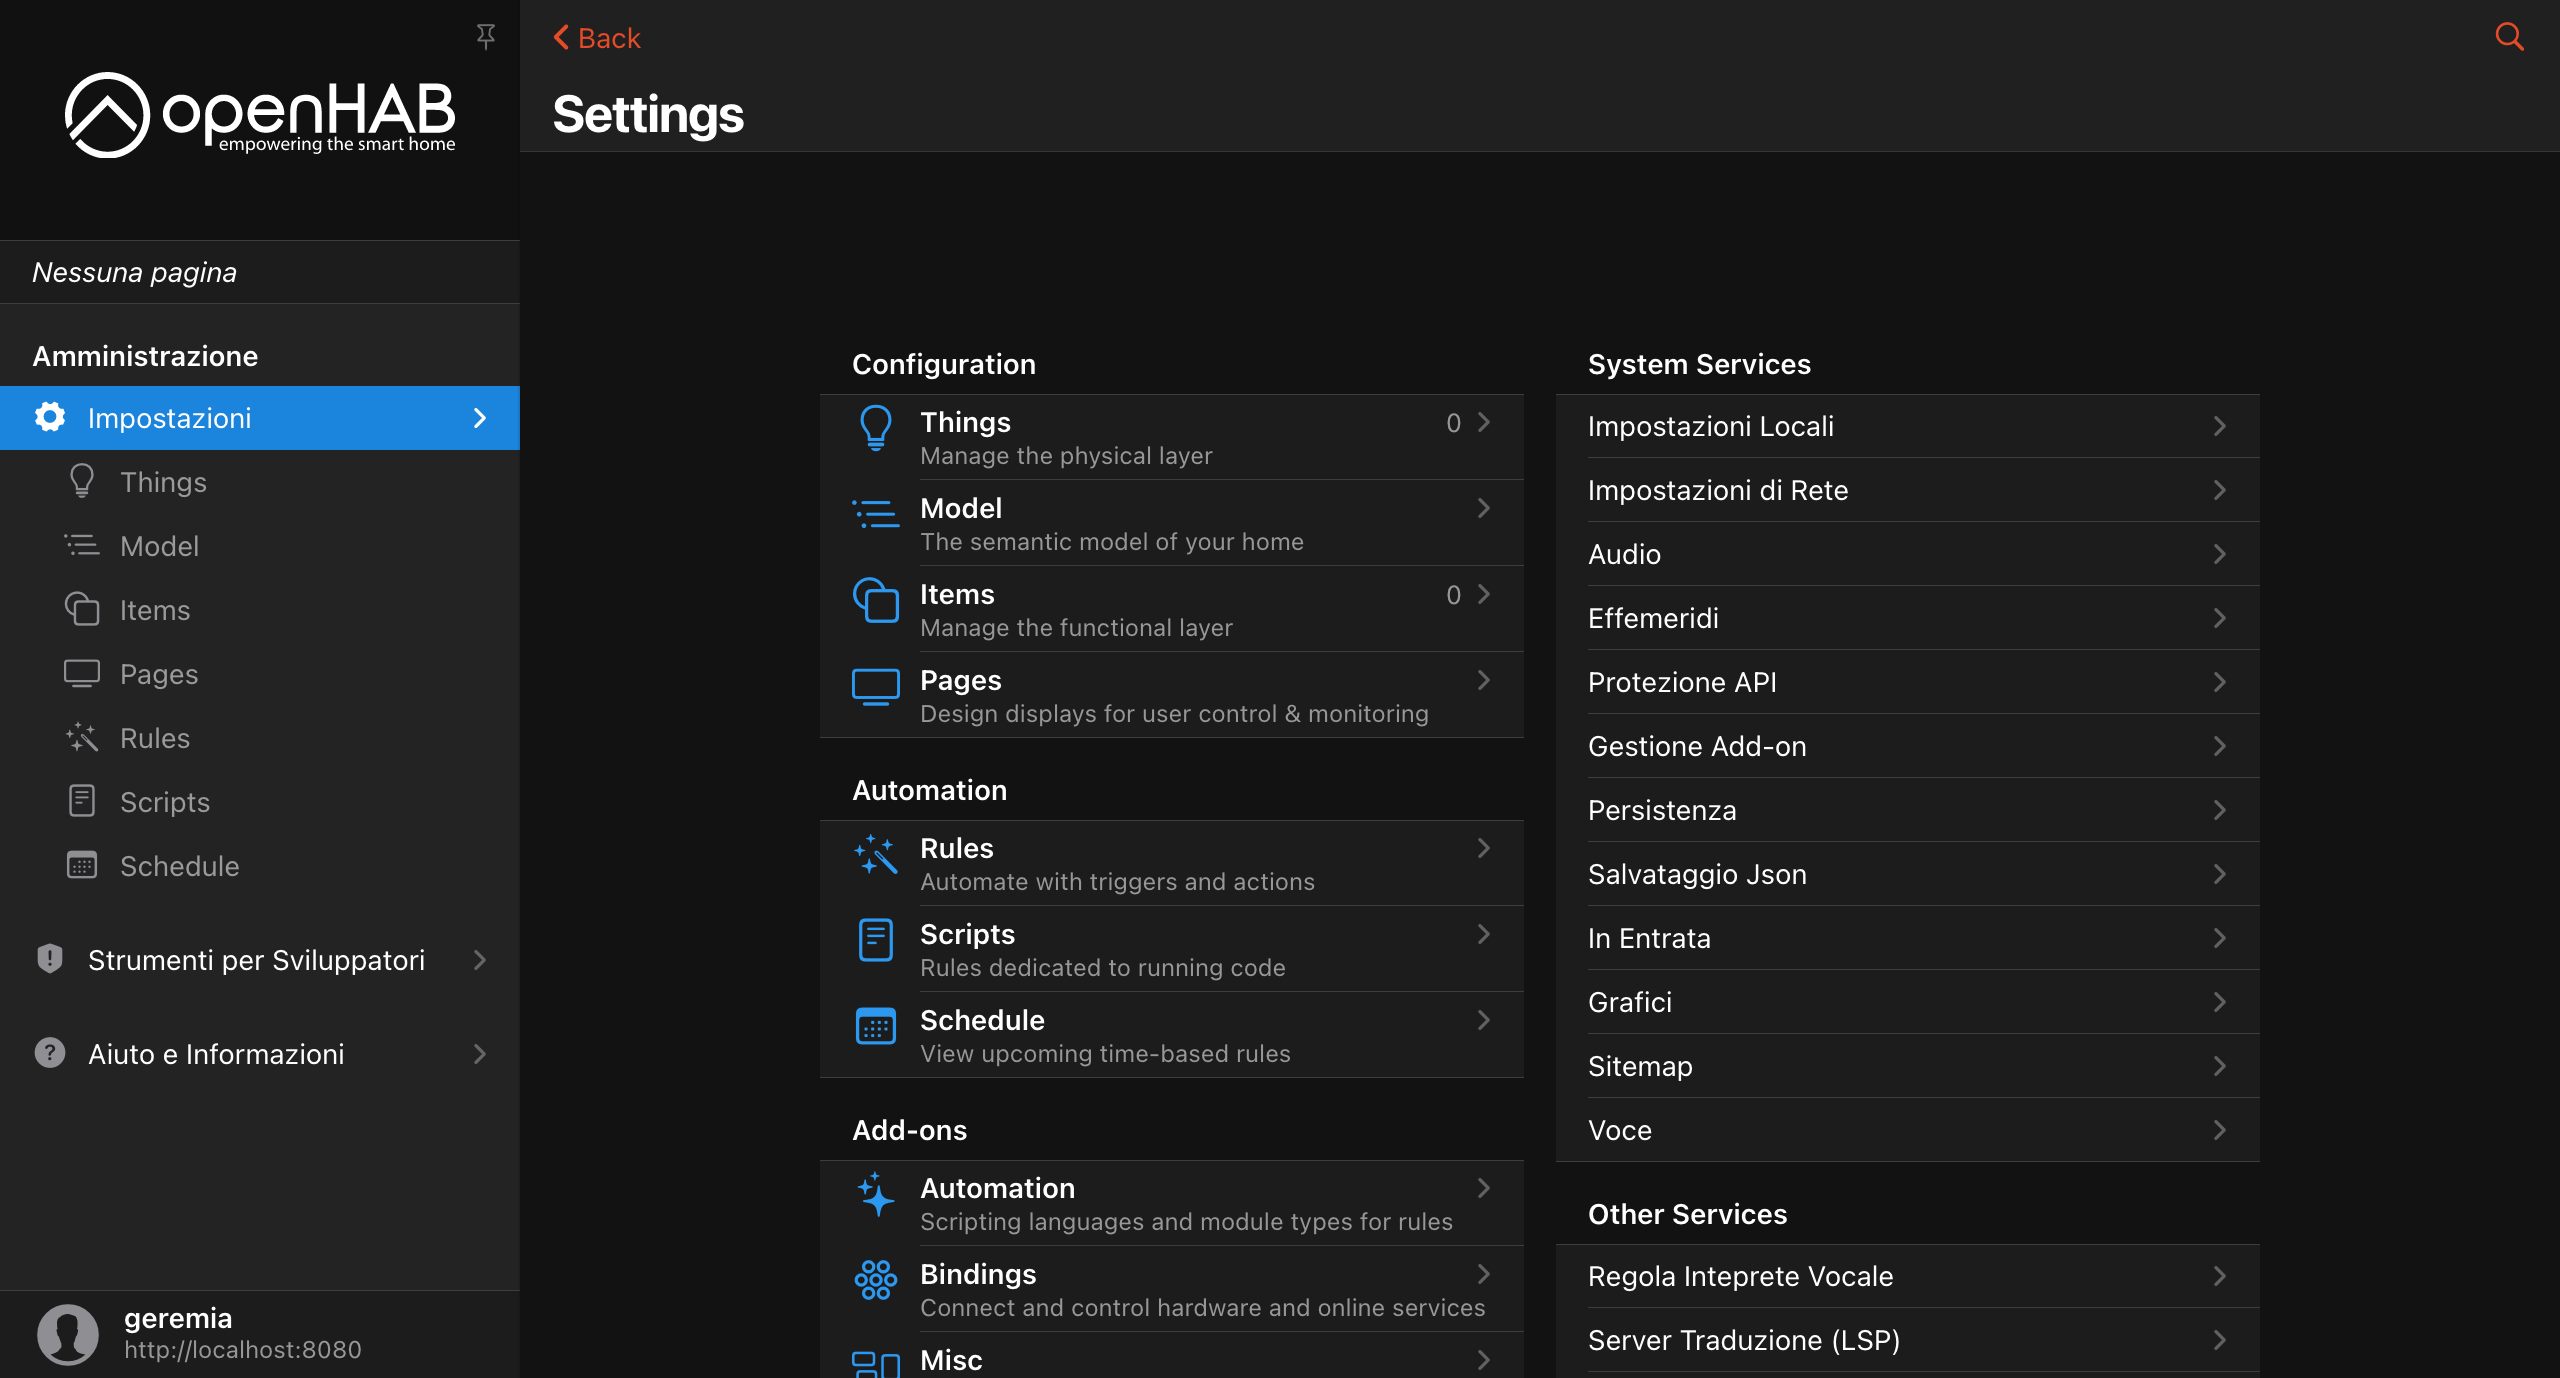
\includegraphics[width=12cm]{Immagini/schermata_impostazioni}
        \caption{Schermata Impostazioni}
        \label{fig:schermata_impostazioni}
    \end{figure}
    \item \label{enum:plus} premere sul ``+'' in basso a destra per scegliere un binding (Figura \ref{fig:schermata_things})
    \begin{figure}
        \centering
        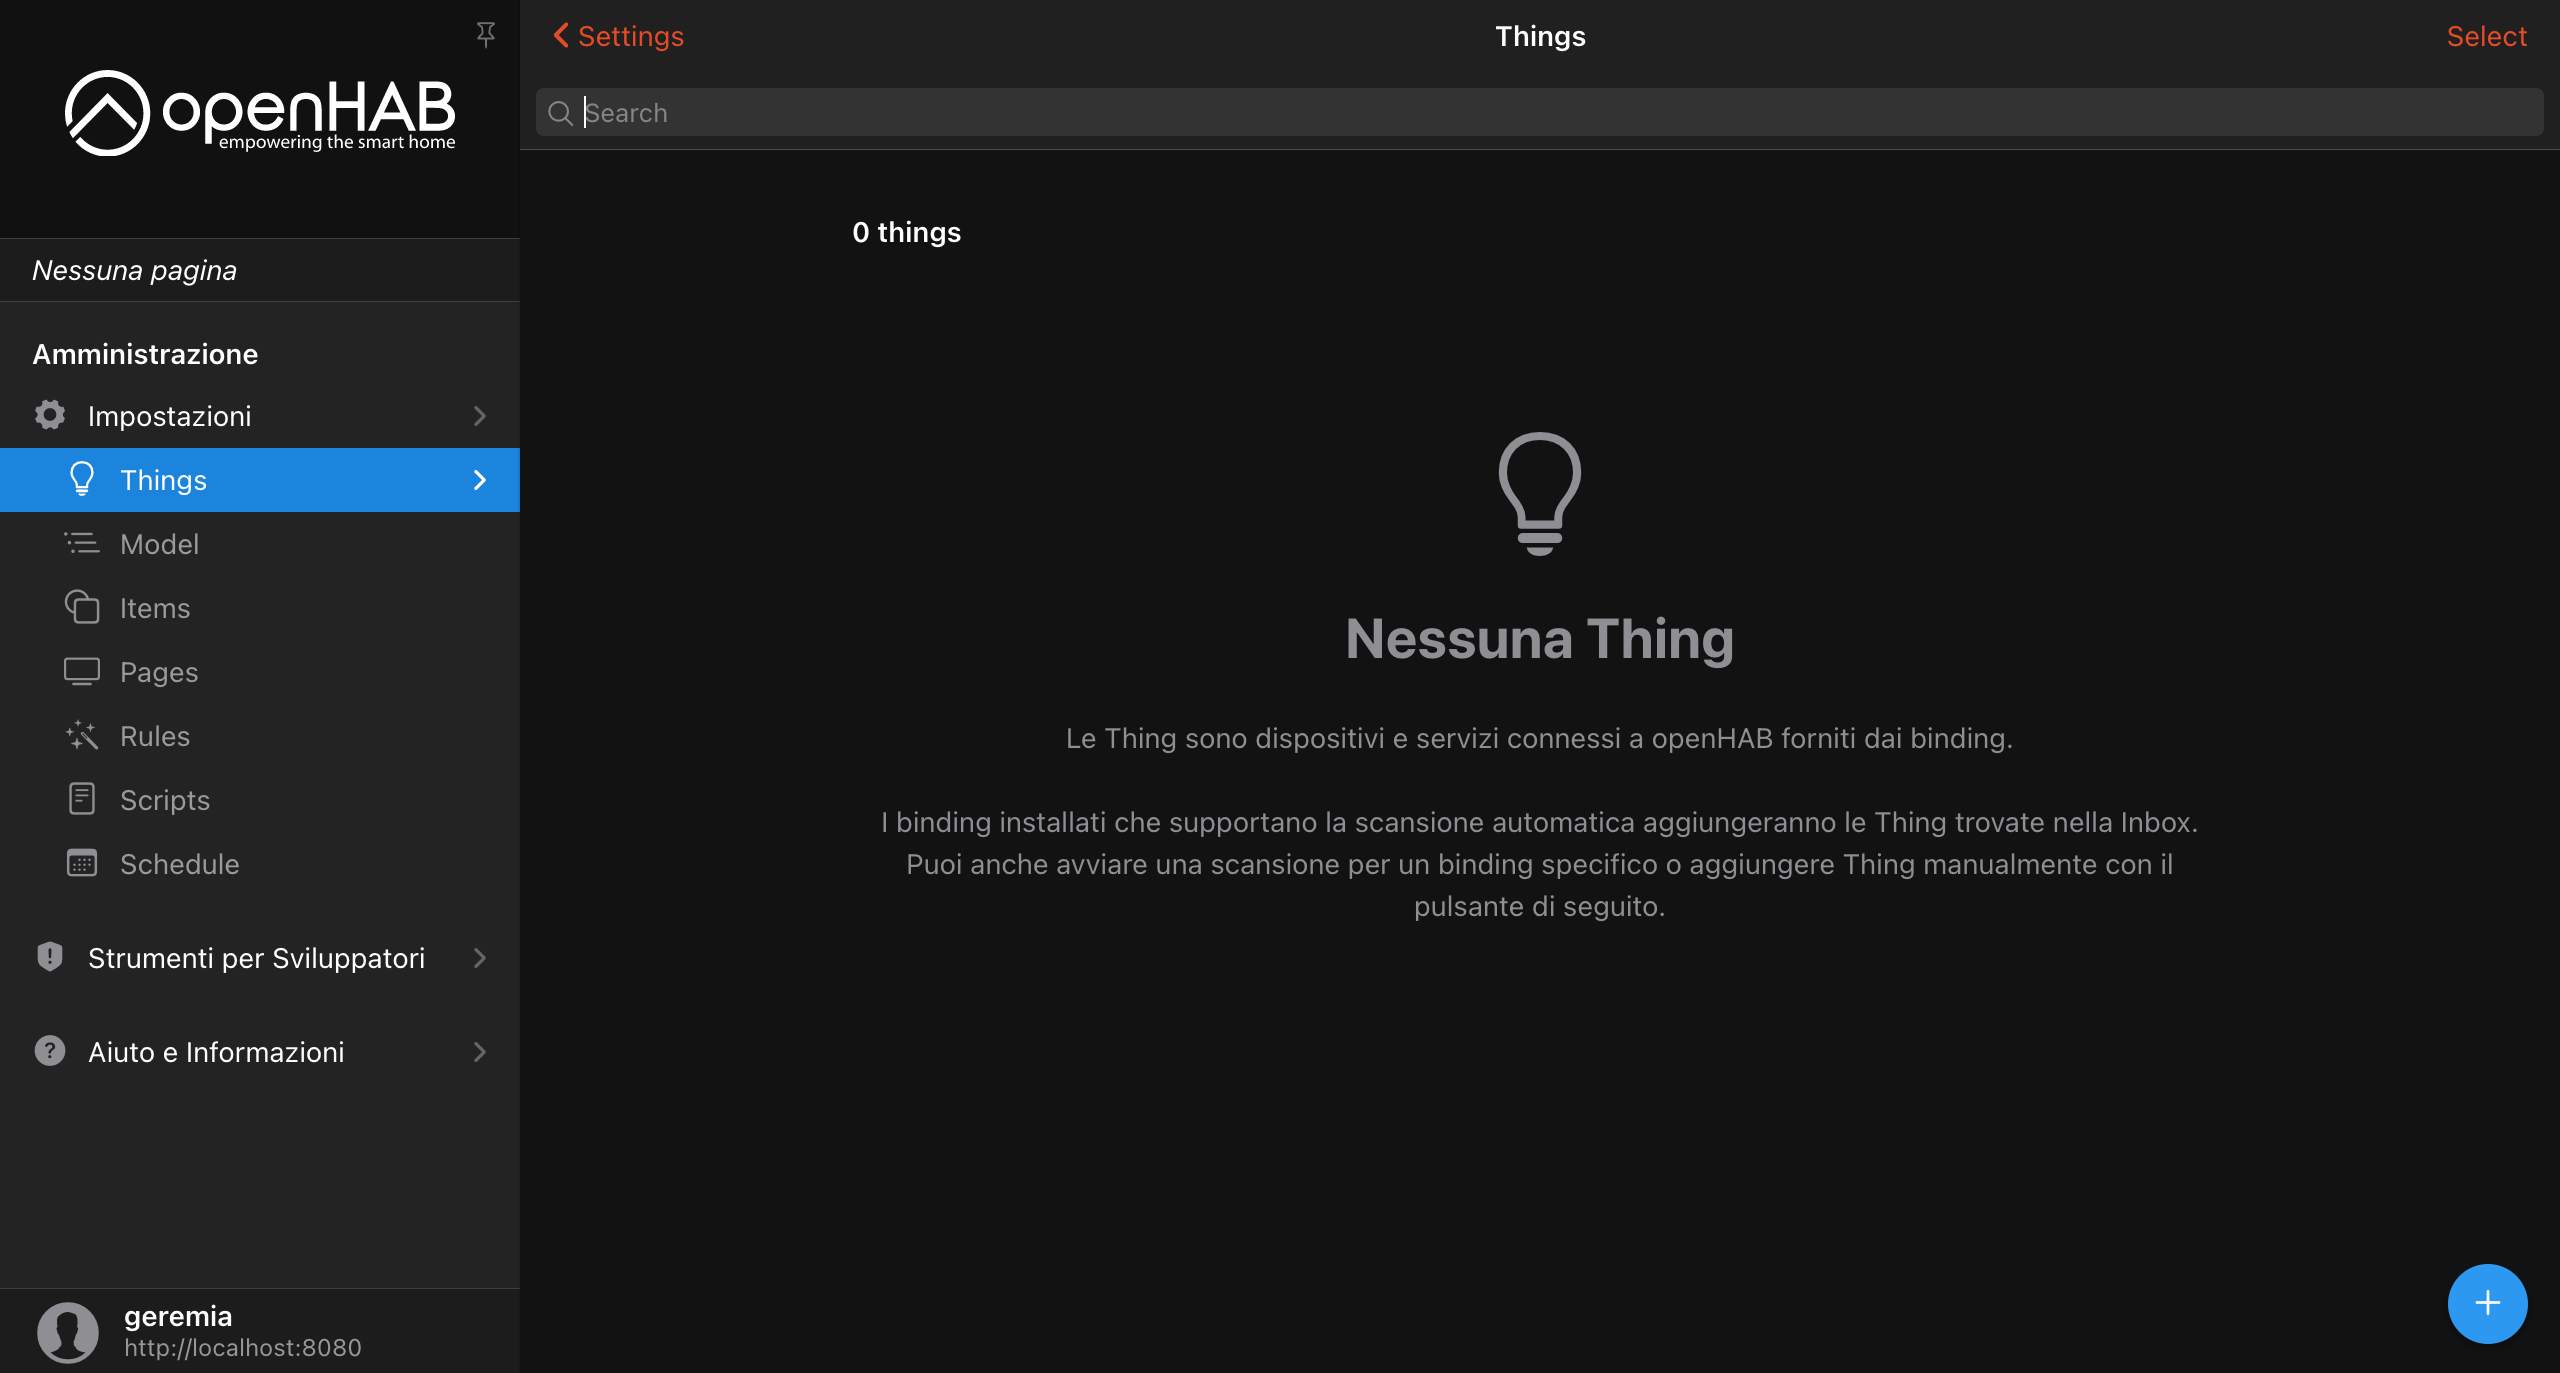
\includegraphics[width=12cm]{Immagini/schermata_things}
        \caption{Schermata Things}
        \label{fig:schermata_things}
    \end{figure}
    \item \label{enum:mqtt_binding}  scegliere il ``MQTT binding'' (Figura \ref{fig:choose_binding})
    \begin{figure}
        \centering
        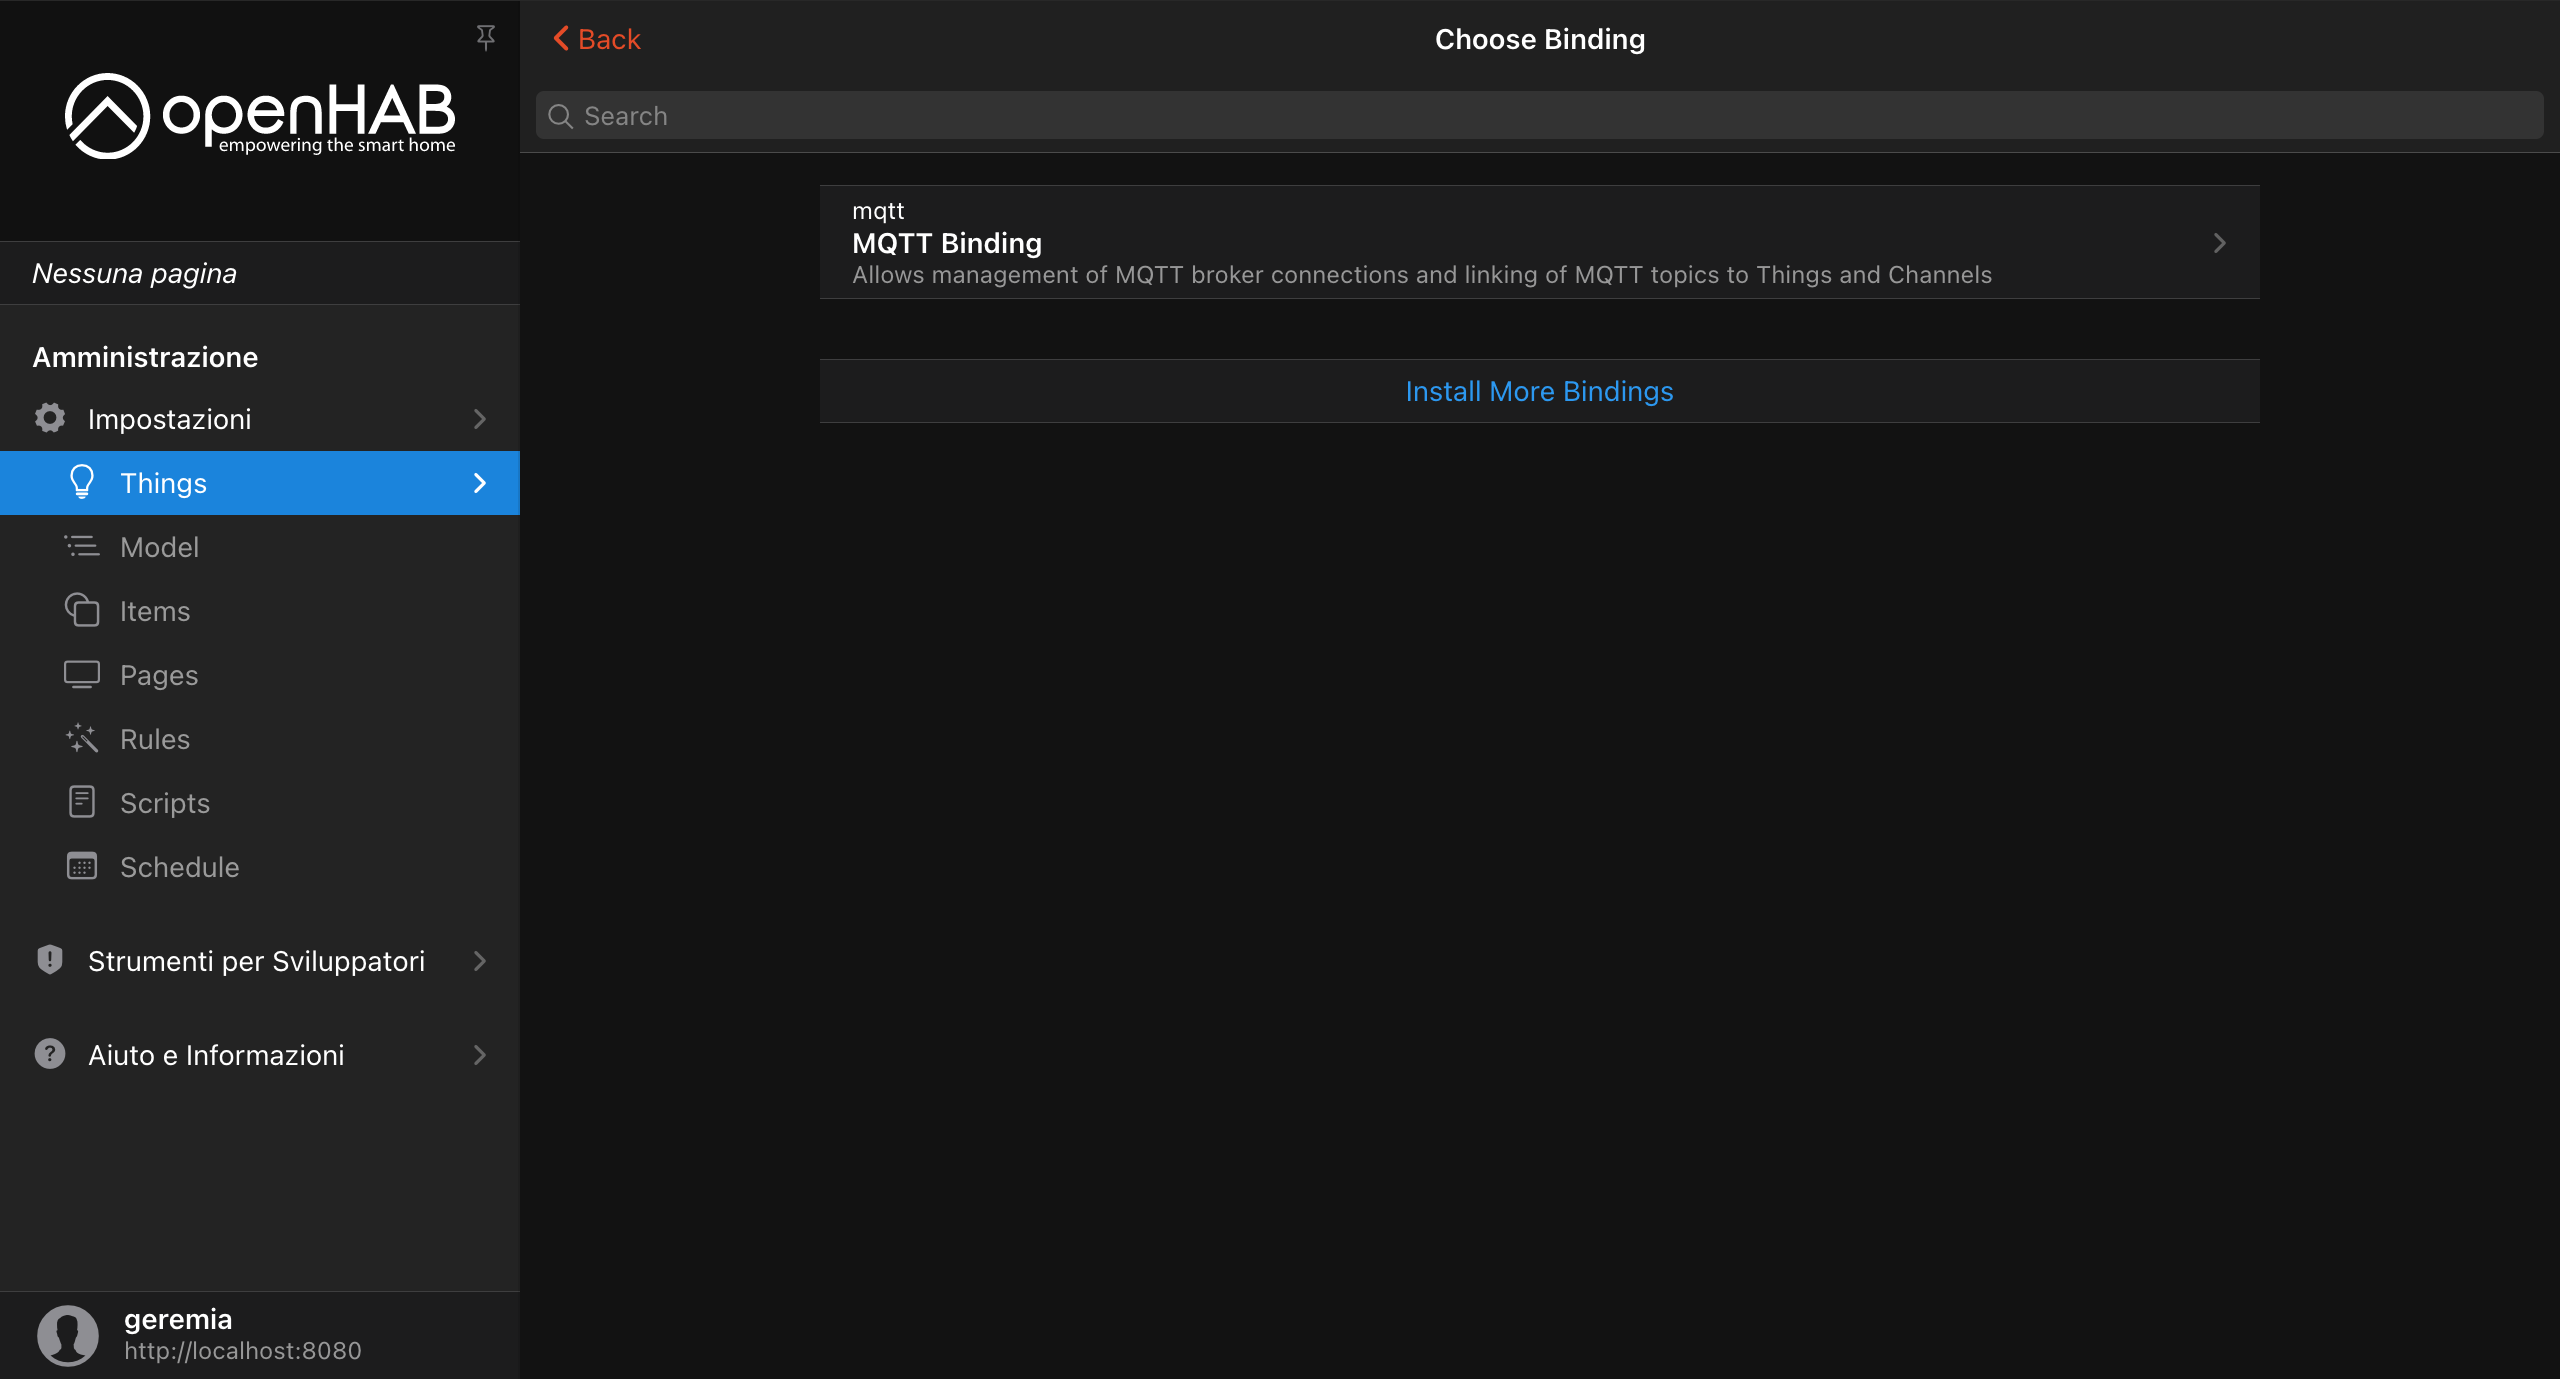
\includegraphics[width=12cm]{Immagini/choose_binding}
        \caption{Schermata Scelta Binding}
        \label{fig:choose_binding}
    \end{figure}
    \item aggiungere la thing ``MQTT Broker'' (Figura \ref{fig:add_new_thing})
    \begin{figure}
        \centering
        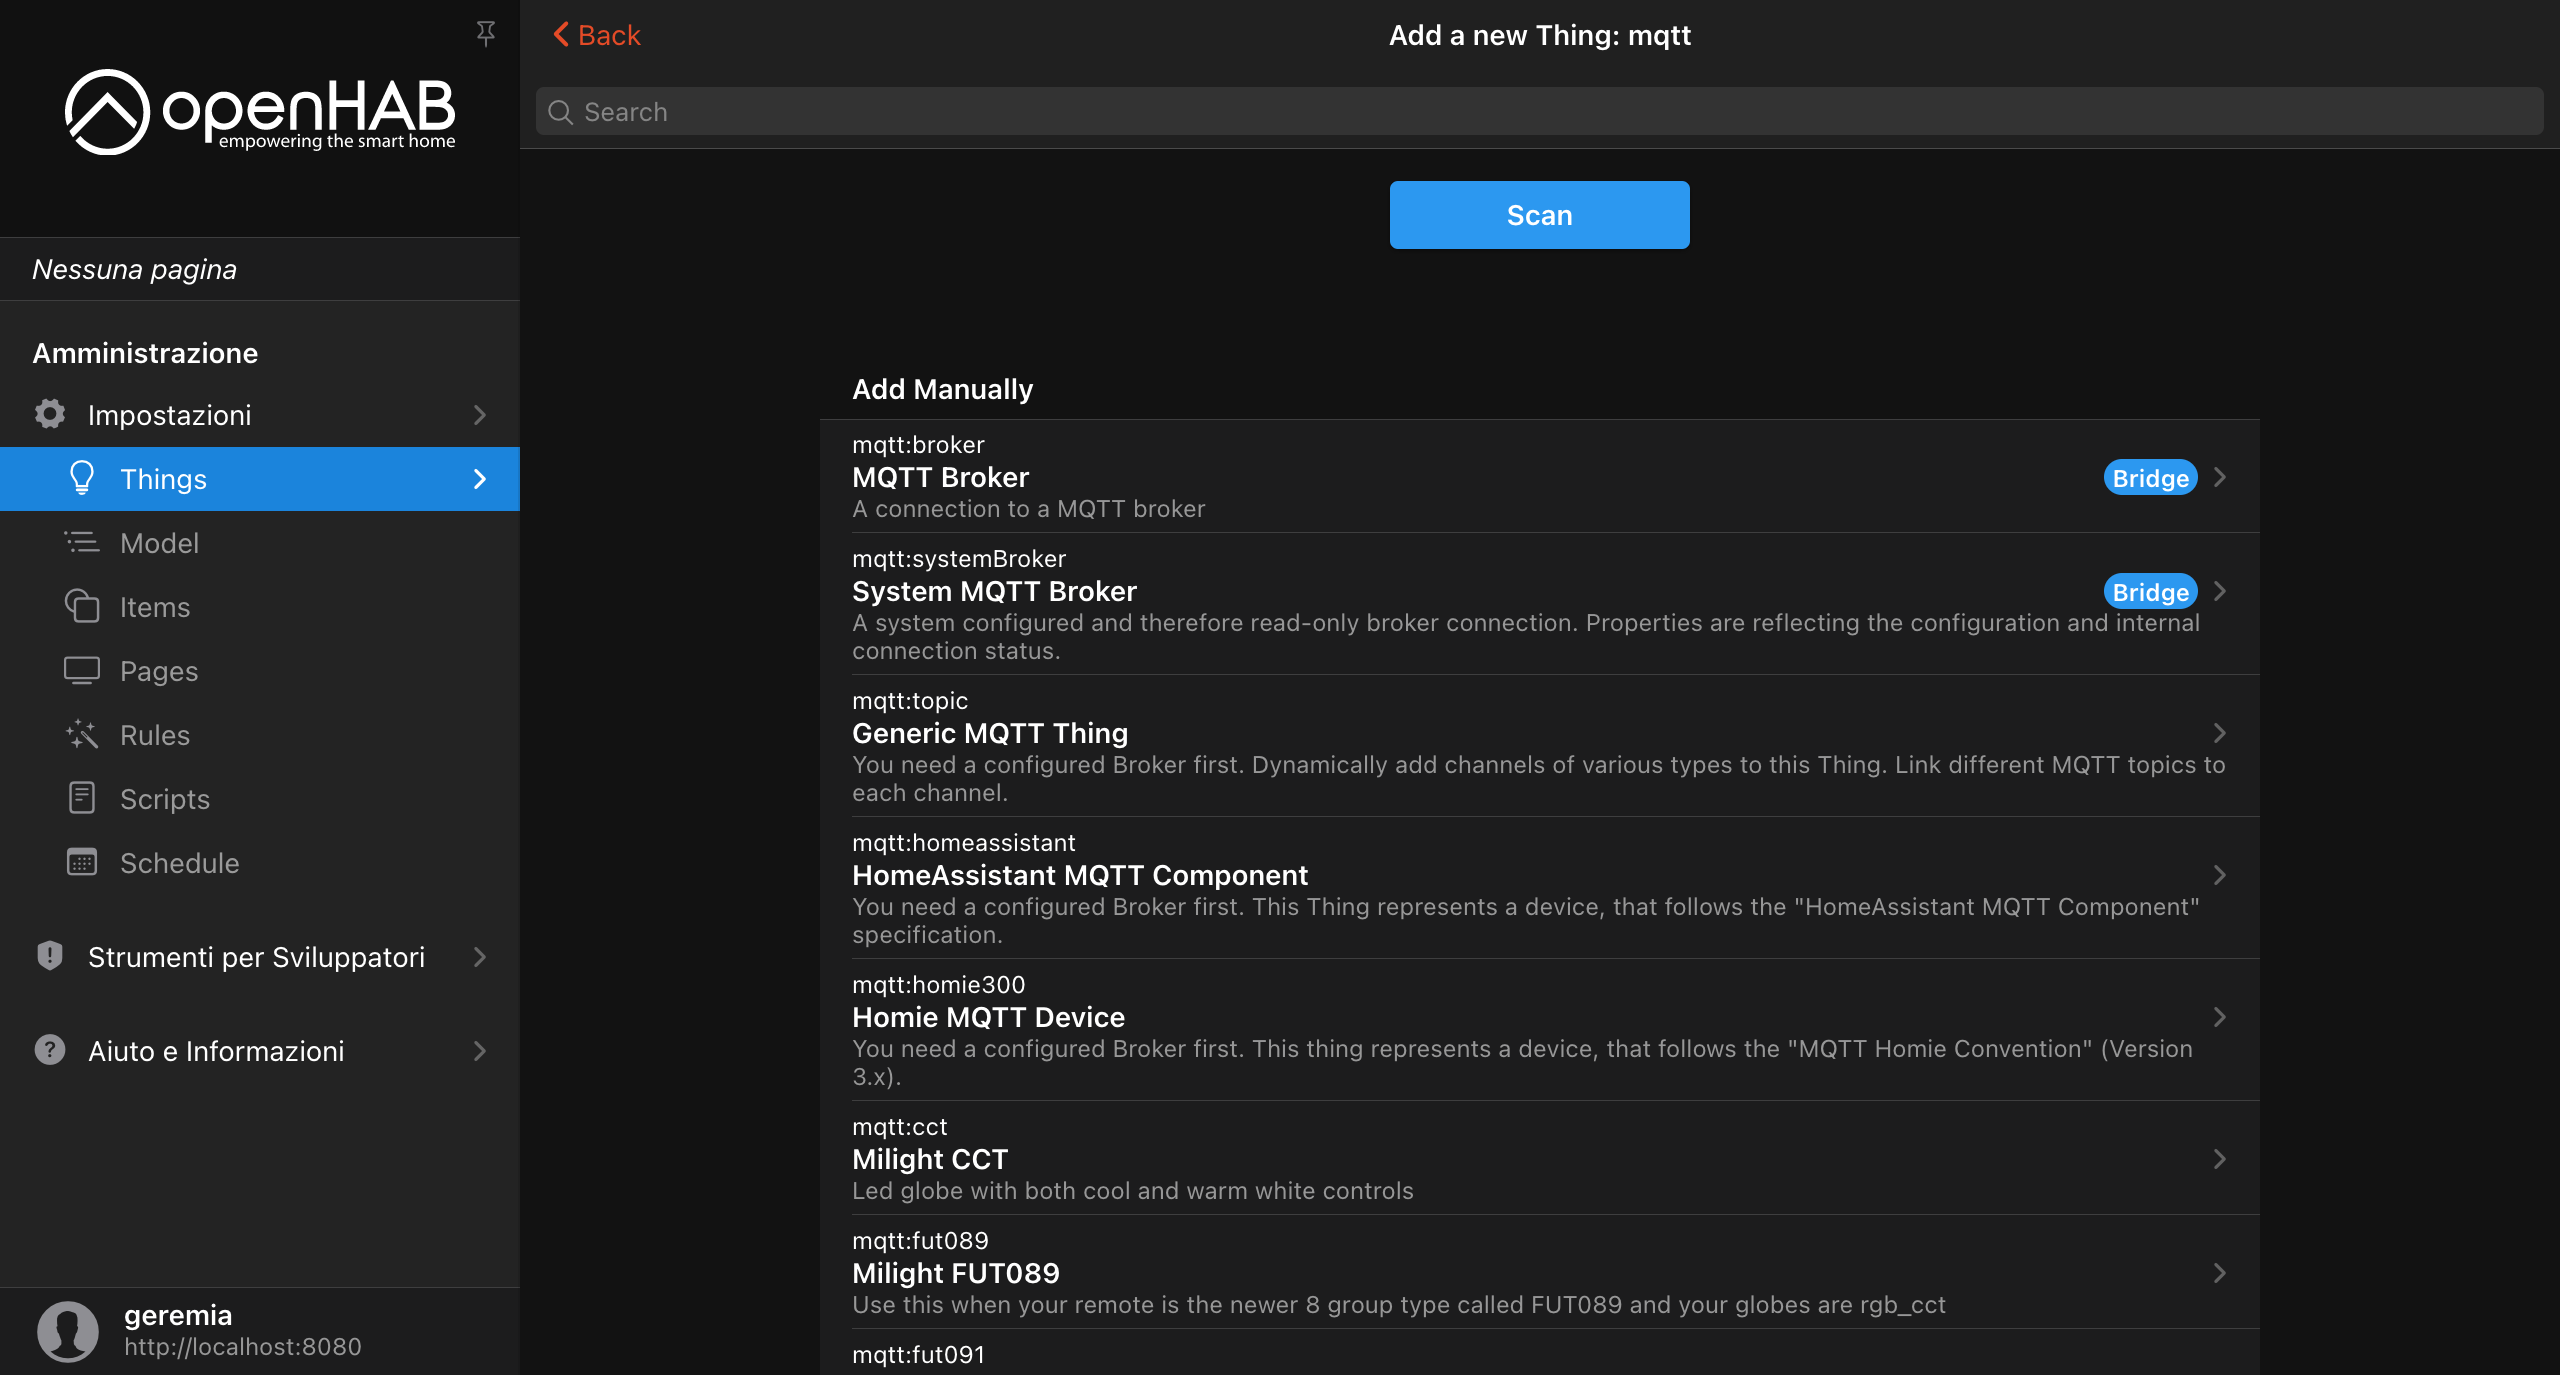
\includegraphics[width=12cm]{Immagini/add_new_thing}
        \caption{Schermata aggiunta Thing}
        \label{fig:add_new_thing}
    \end{figure}
    \item \label{enum:mqtt_broker} configurare {\em MQTT Broker} aggiungendo {\em Broker Hostname/IP} (IP del broker MQTT) e premendo sul pulsante ``Create Thing'' (in tal caso verr\'a aggiunto l'indirizzo IP locale della Raspberry Pi che ha gi\'a mosquitto installato). Appena eseguita tale operazione si ritorner\'a alla schermata precedente con la nuova thing aggiunta. In tale schermata \'e possibile visualizzare se lo stato del broker MQTT \'e ONLINE o OFFLINE 
    (Figura \ref{fig:mqtt_broker_config})
    \begin{figure}
        \centering
        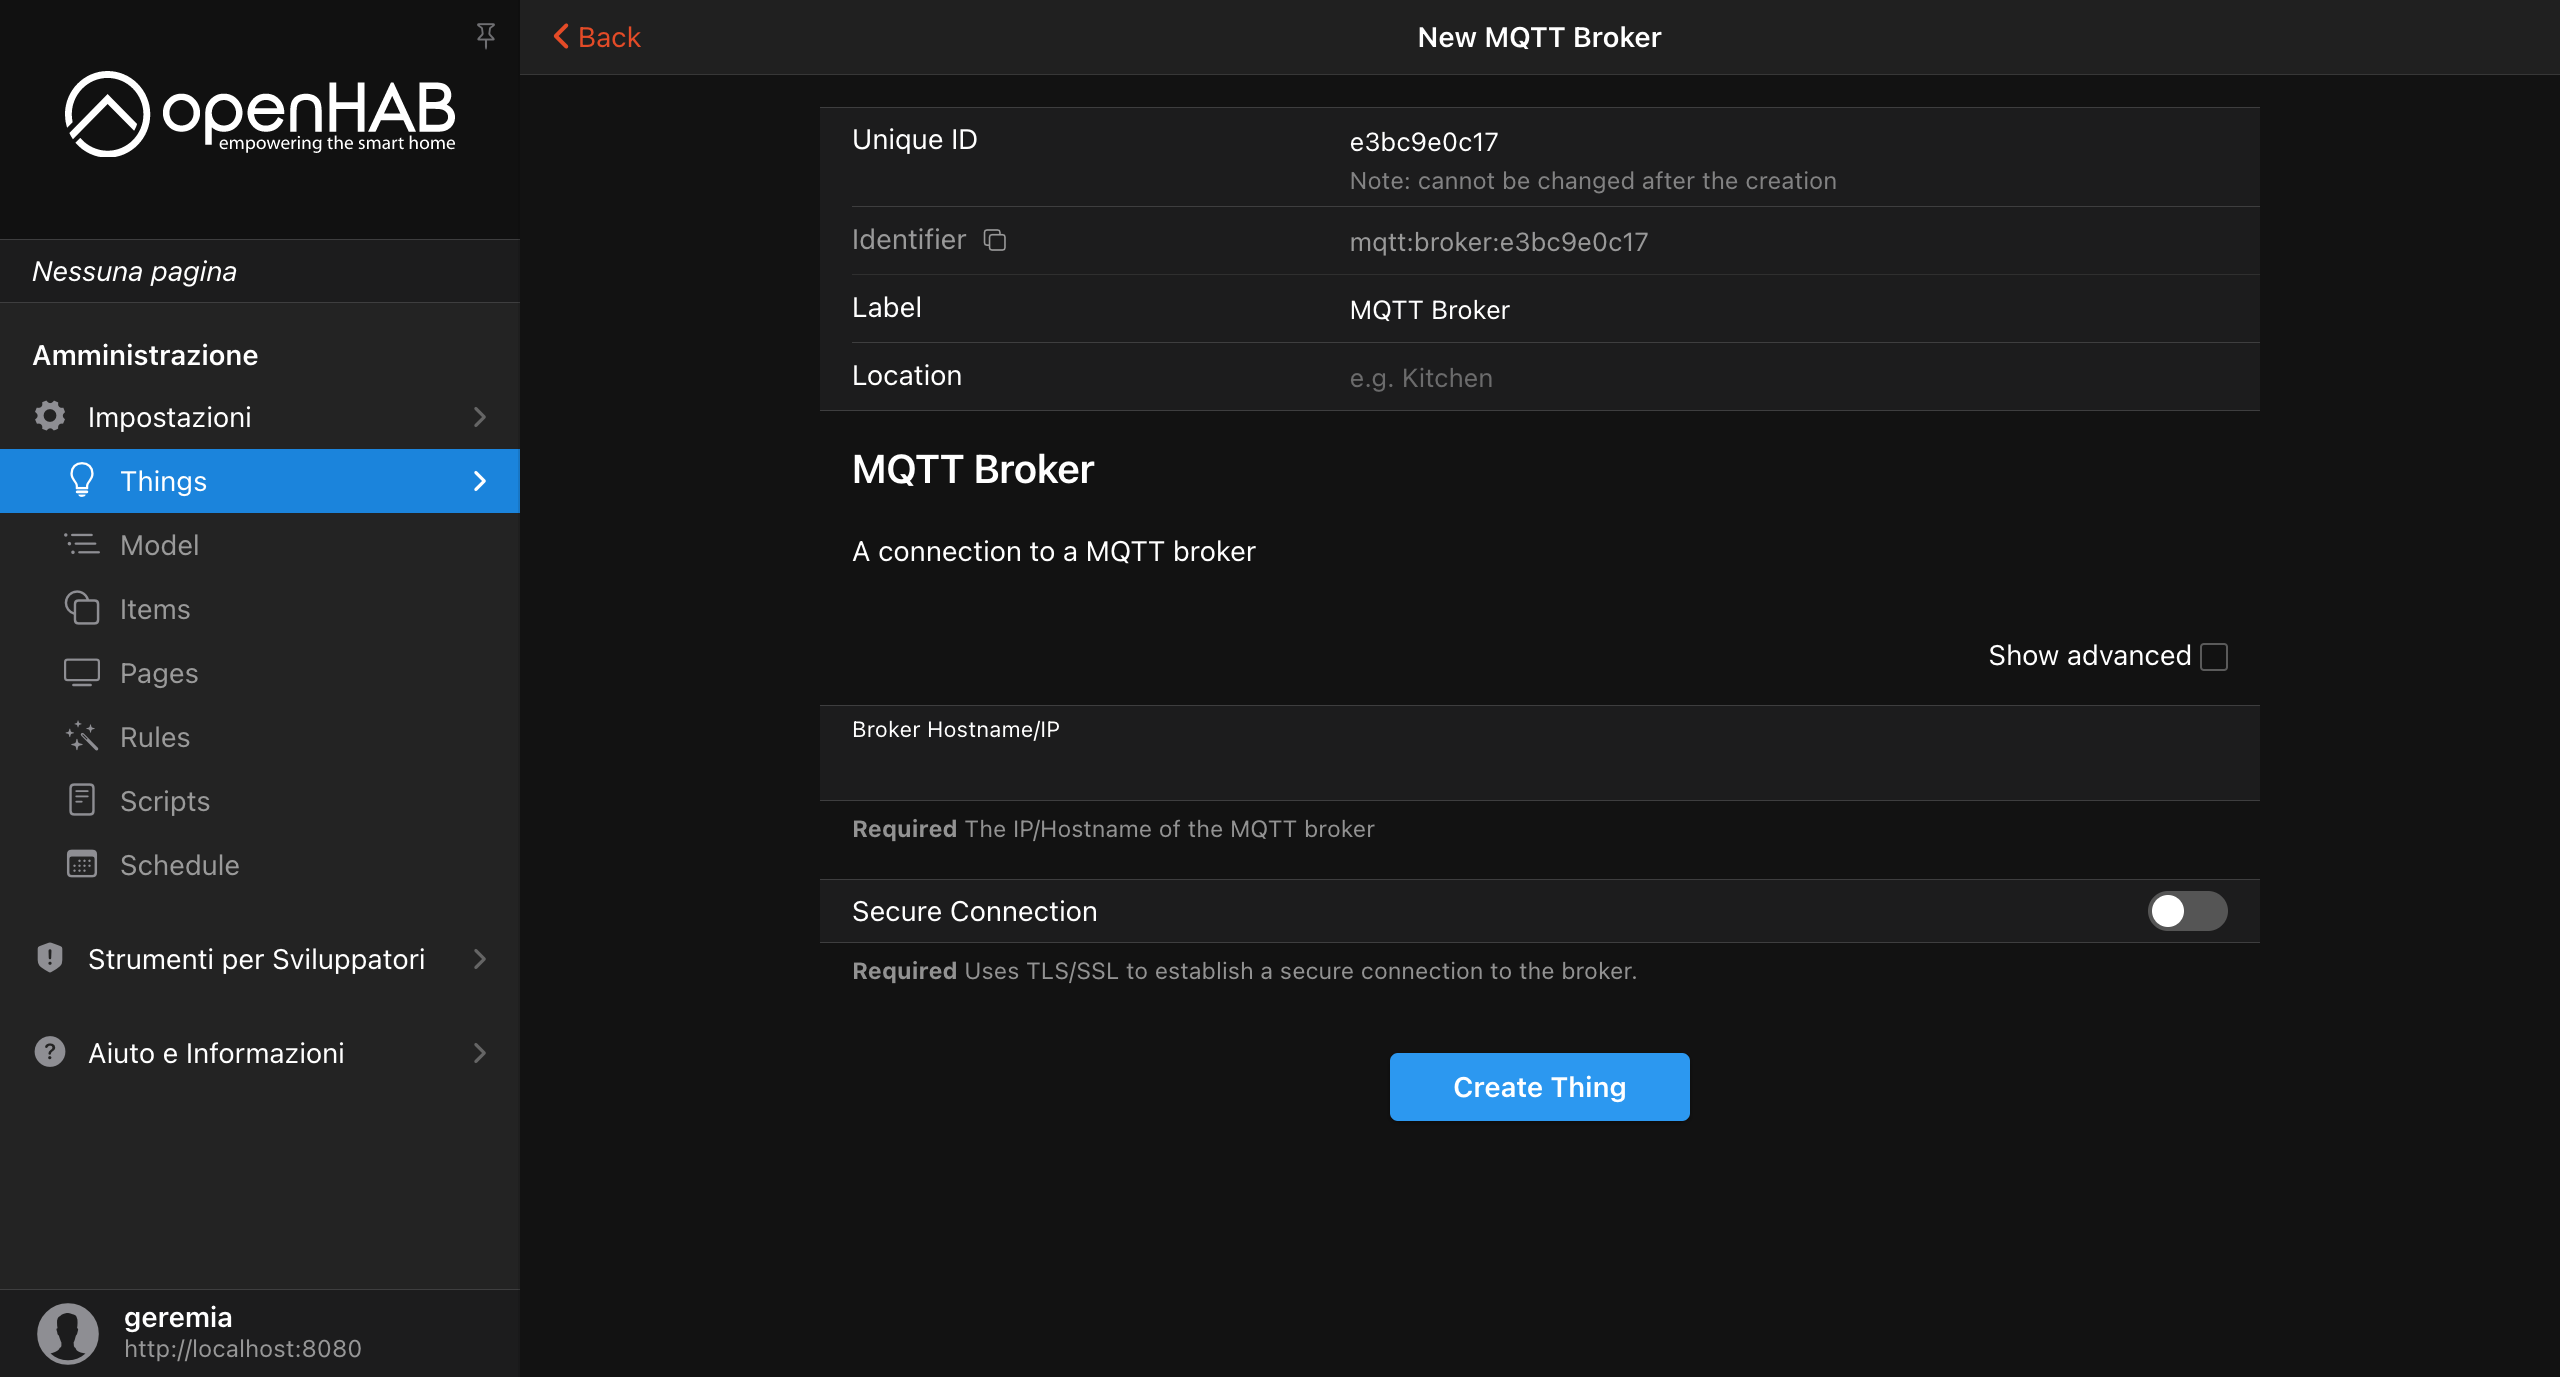
\includegraphics[width=12cm]{Immagini/mqtt_broker_config}
        \caption{Configurazione MQTT Broker}
        \label{fig:mqtt_broker_config}
    \end{figure}
    \item aggiungere un ulterioire thing rieseguendo i passaggi \ref{enum:plus} e \ref{enum:mqtt_binding} e selezionando questa volta la voce ``Generic MQTT Thing''
    \item si procede alla configurazione aggiungendo i campi:
    \begin{itemize}
        \item \textbf{Label}: rinominarlo con un nome mnemonico cos\'i da rendere pi\'u semplice la sua ricerca futura (in questo caso ``Samrt Garden'')
        \item \textbf{Location}: aggiungere la posizione nella casa della nuova thing (in questo caso ``Garden'')
        \item \textbf{Bridge}: selezionare ``MQTT Broker'', ovvero la thing aggiunta al passaggio \ref{enum:mqtt_broker}
    \end{itemize}
    premere infine su ``Create Thing'' (Figura \ref{fig:mqtt_thing_config})
    \begin{figure}
        \centering
        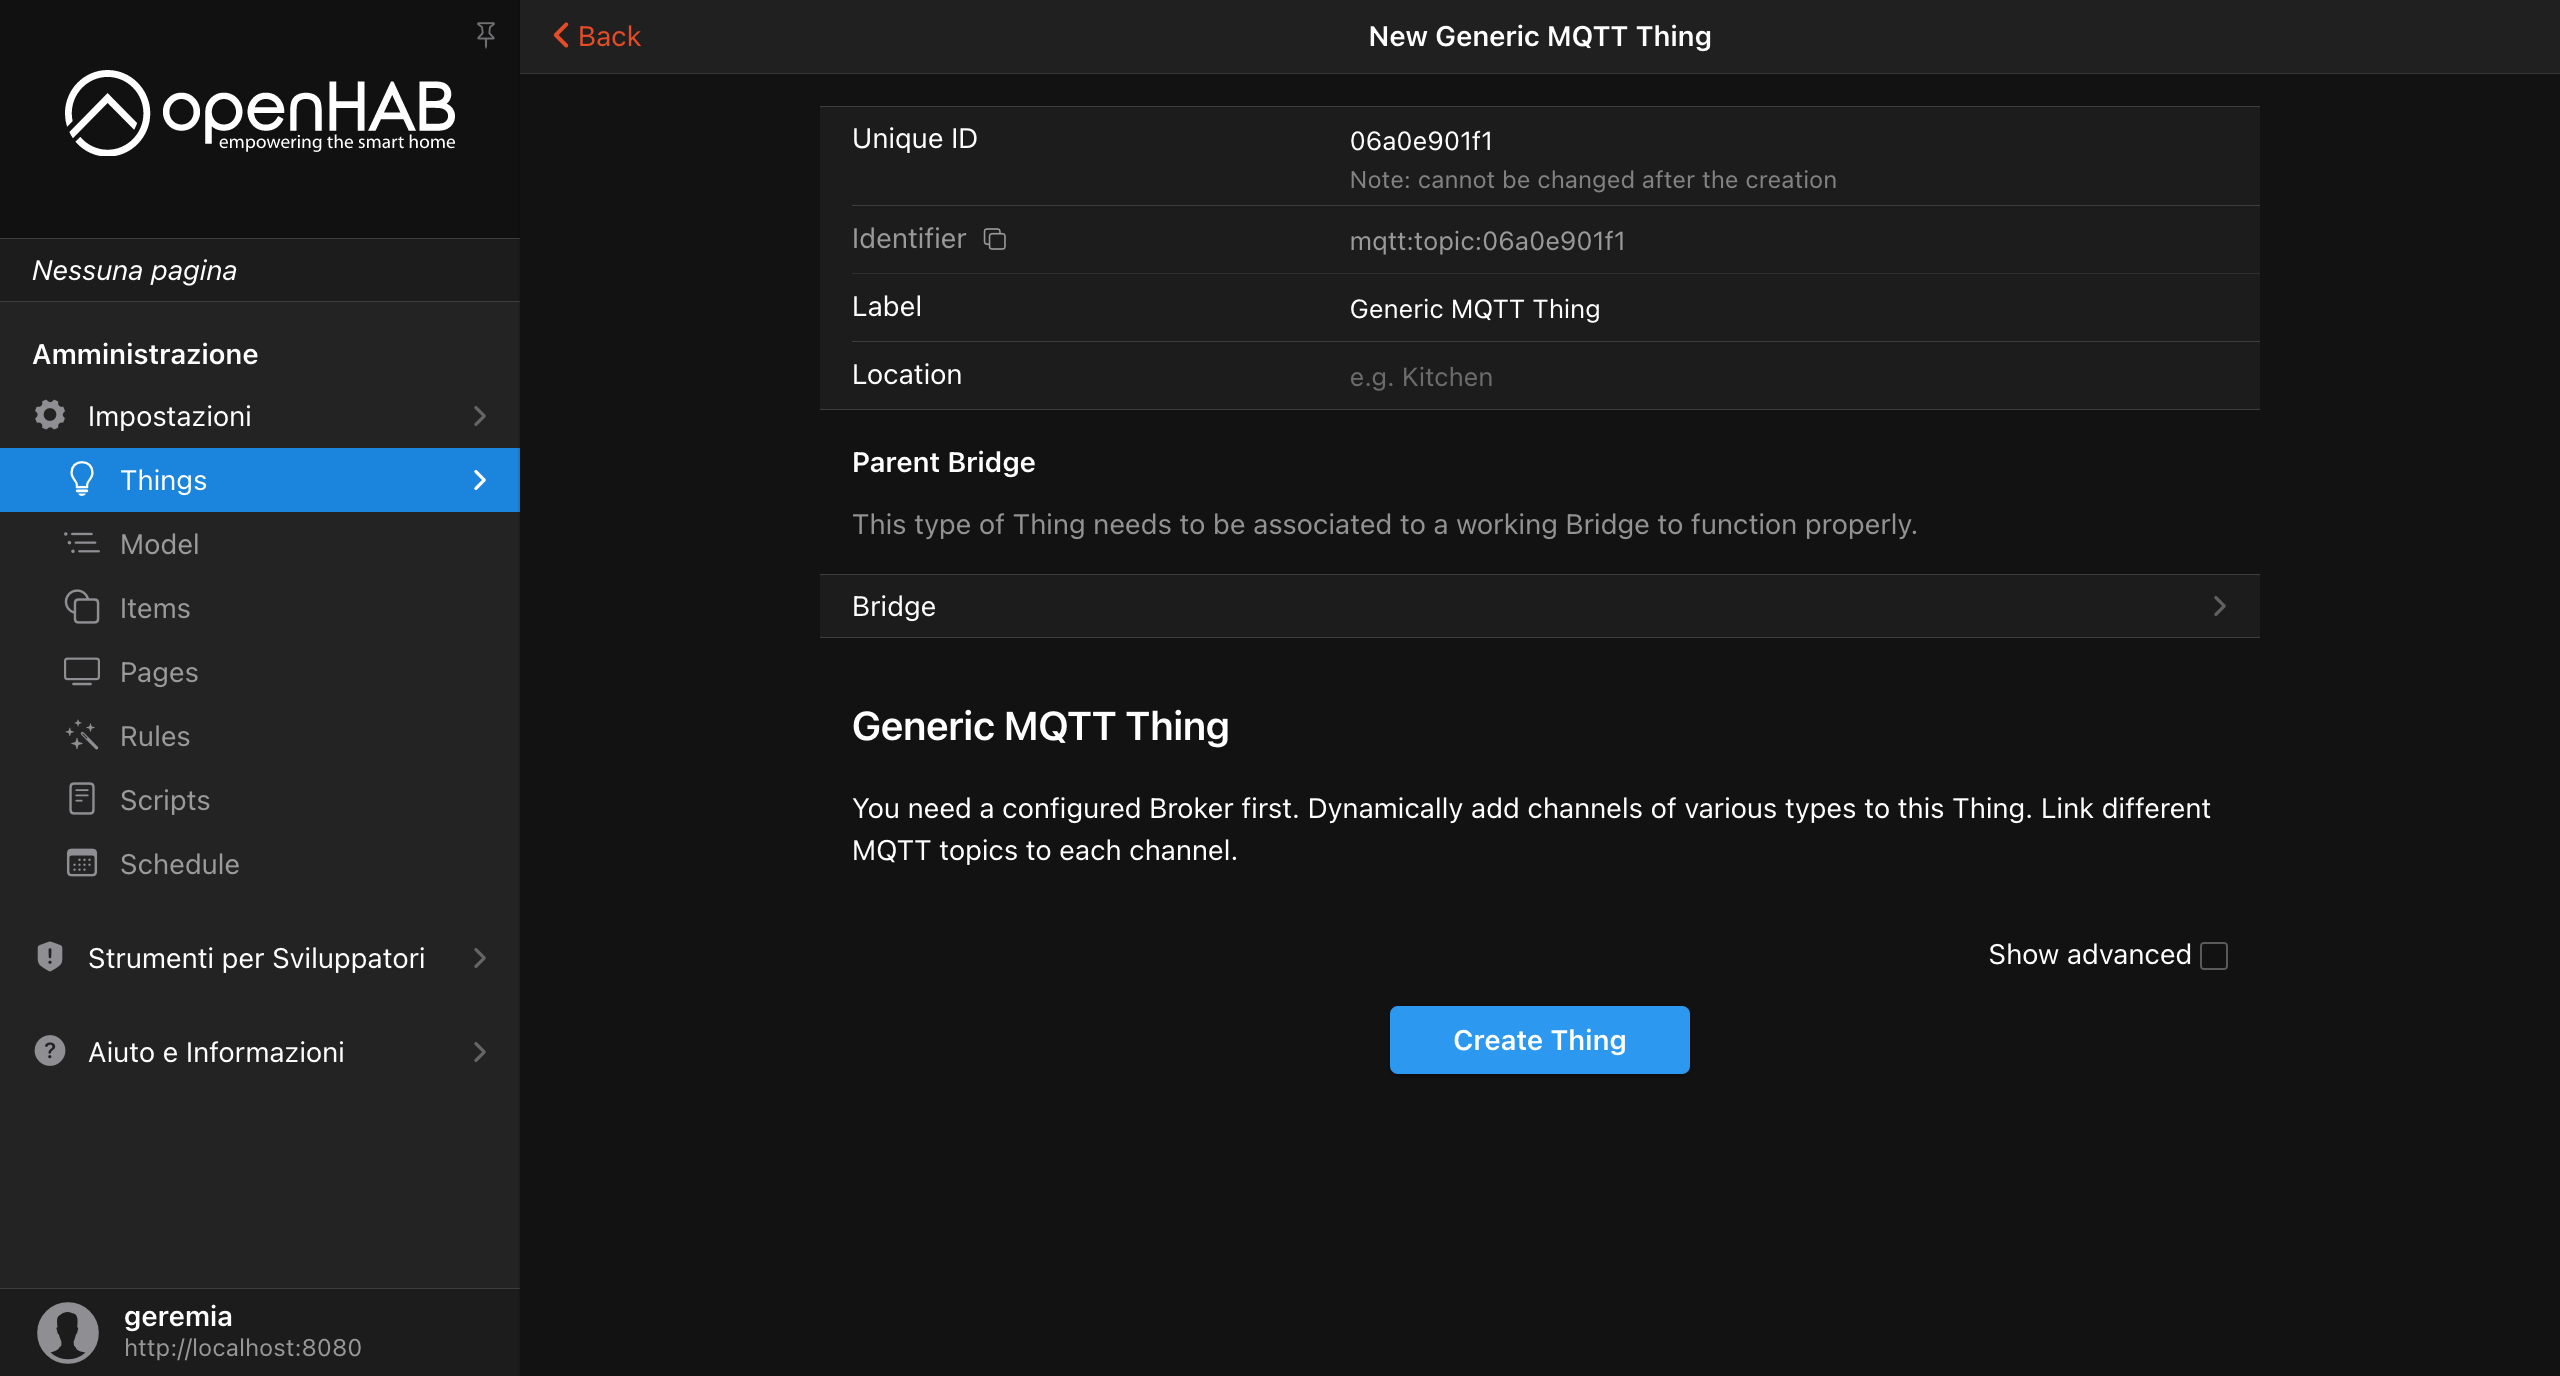
\includegraphics[width=12cm]{Immagini/mqtt_thing_config}
        \caption{Configurazione MQTT Thing}
        \label{fig:mqtt_thing_config}
    \end{figure}
    \item ritornati alla schermata Things, a questo punto bisogna aggiungere i Channels relativi ai topic MQTT all'interno della thing appena creata. Quindi premere sulla nuova thing (in questo caso chiamata ``Smart Garden'') e successivamente su Channels. Nella schermata della thing \'e possibile visualizzare il suo status (Figura: \ref{fig:mqtt_thing_smart_garden})
    \begin{figure}
        \centering
        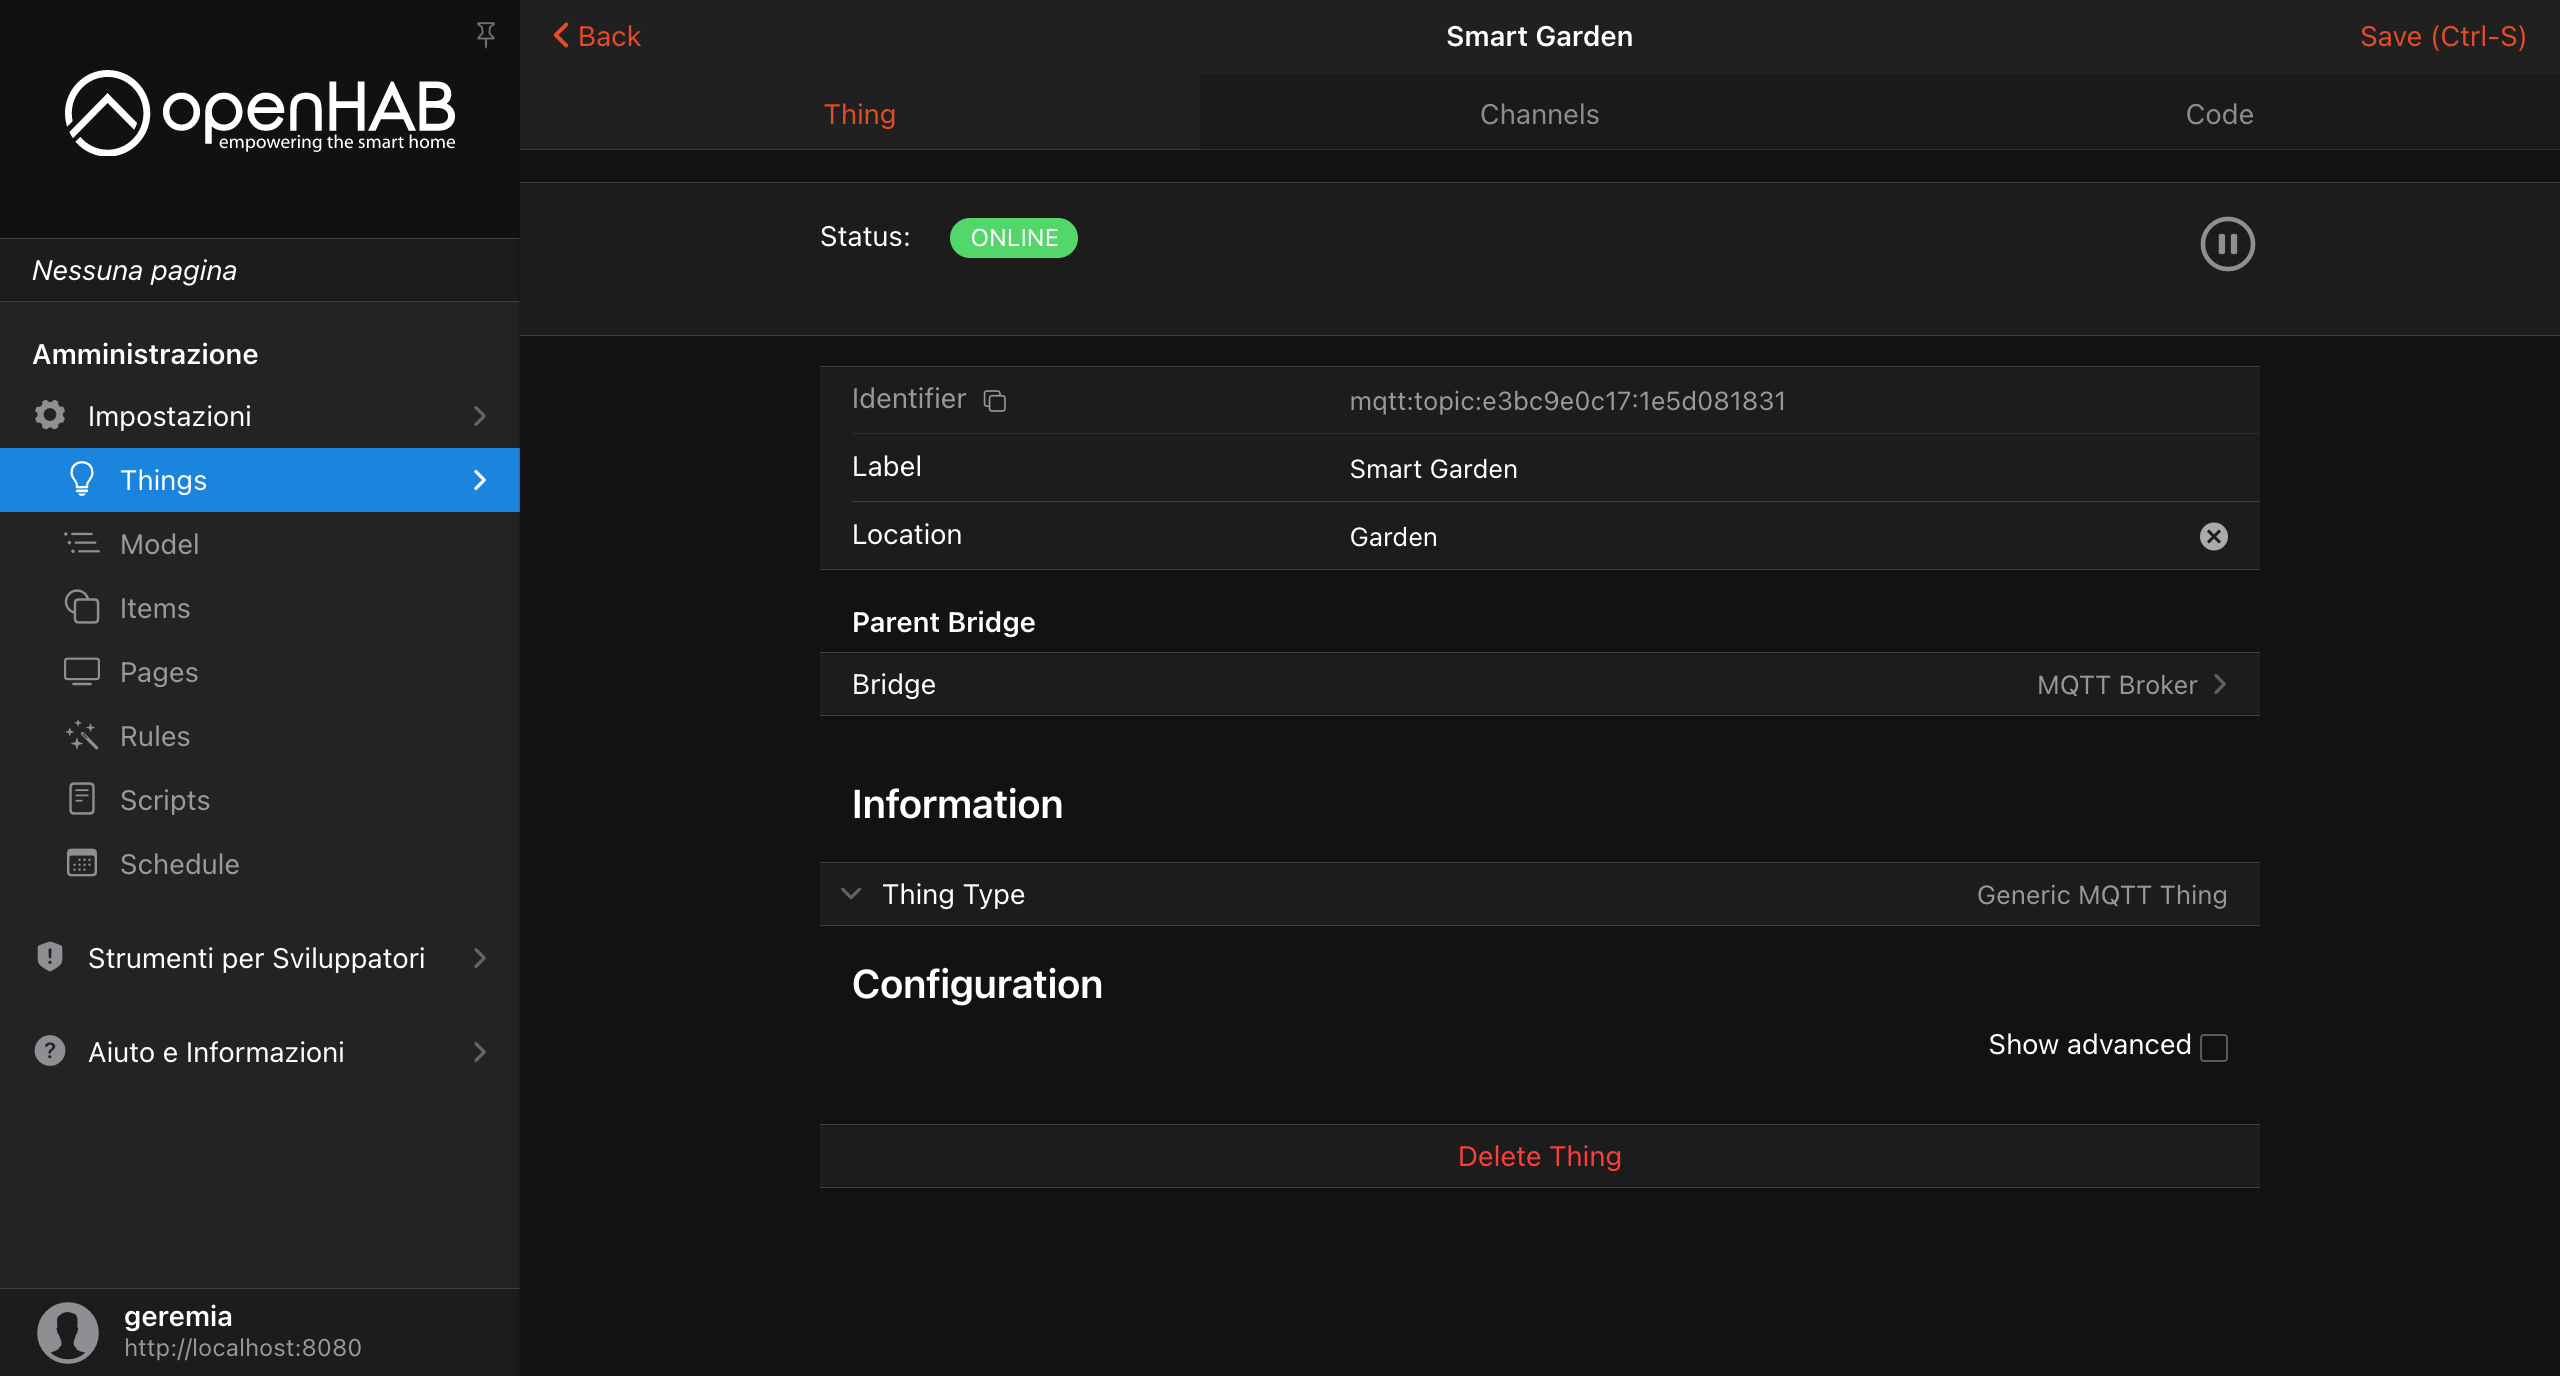
\includegraphics[width=12cm]{Immagini/mqtt_thing_smart_garden}
        \caption{MQTT Thing}
        \label{fig:mqtt_thing_smart_garden}
    \end{figure}
    \item nella schermata Channels \'e possibile aggiungere diversi canali relativi alla thing selezionata precedentamente. Per fare ci\'o basta premere sul pulsante ``Add Channel'' (Figura \ref{fig:channels}) e configurare il channel da aggiungere inserendo i campi richiesti:
    \begin{itemize}
        \item \textbf{Channel Identifier}: id univoco del channel
        \item \textbf{Label}: nome con cui verr\'a visualizzato a video il canale
        \item \textbf{Channel Type}: tipo del channel. Da questo usciranno fuori poi altri campi relativi alla sua configurazione
    \end{itemize}
    In questo caso sono stati aggiunti 4 channels relativi ad ogni topic(handle\_pump e status\_pump fanno riferimento allo stesso topic in due modi differenti: il primo serve per gestire la pompe in maniera manuale accendendola e spegnendola mentre il secondo per visualizzare il suo stato). Verranno riportati con le relative configurazioni alla Tabella \ref{tab:smart_garden_channels}. In quest'ultima i campi ON e OFF sono relativi solo al tipo ``On/Off Switch'' poich\'e corrispondono alle azioni di accenzione e spegnimento. In tutti i channels pu\'o essere attivata la voce sotto ``Show advanced'' chiamata ``Retained'' per abilitare i messaggi inviati ai relativi topic come mantenuti
    \begin{table}[]
        \centering
        \begin{tabular}{l|l|l|l|l|l}
            \textbf{Identifier} & \textbf{Label} & \textbf{Type} & \textbf{Topic} & \textbf{On} & \textbf{Off} \\
            \hline
            handle\_pump & Handle Pump & On/Off Switch & handle/pump & ON & OFF \\
            handle\_auto & Handle Auto & On/Off Switch & handle/auto & ON & OFF \\
            status\_pump & Status Pump & Text Value & handle/pump & - & - \\
            status\_soil & Status Soil & Text Value & status/soil & - & - \\
        \end{tabular}
        \caption{Smart Garden CHannels}
        \label{tab:smart_garden_channels}
    \end{table}
    (Figura \ref{fig:add_channel})
    \begin{figure}
        \centering
        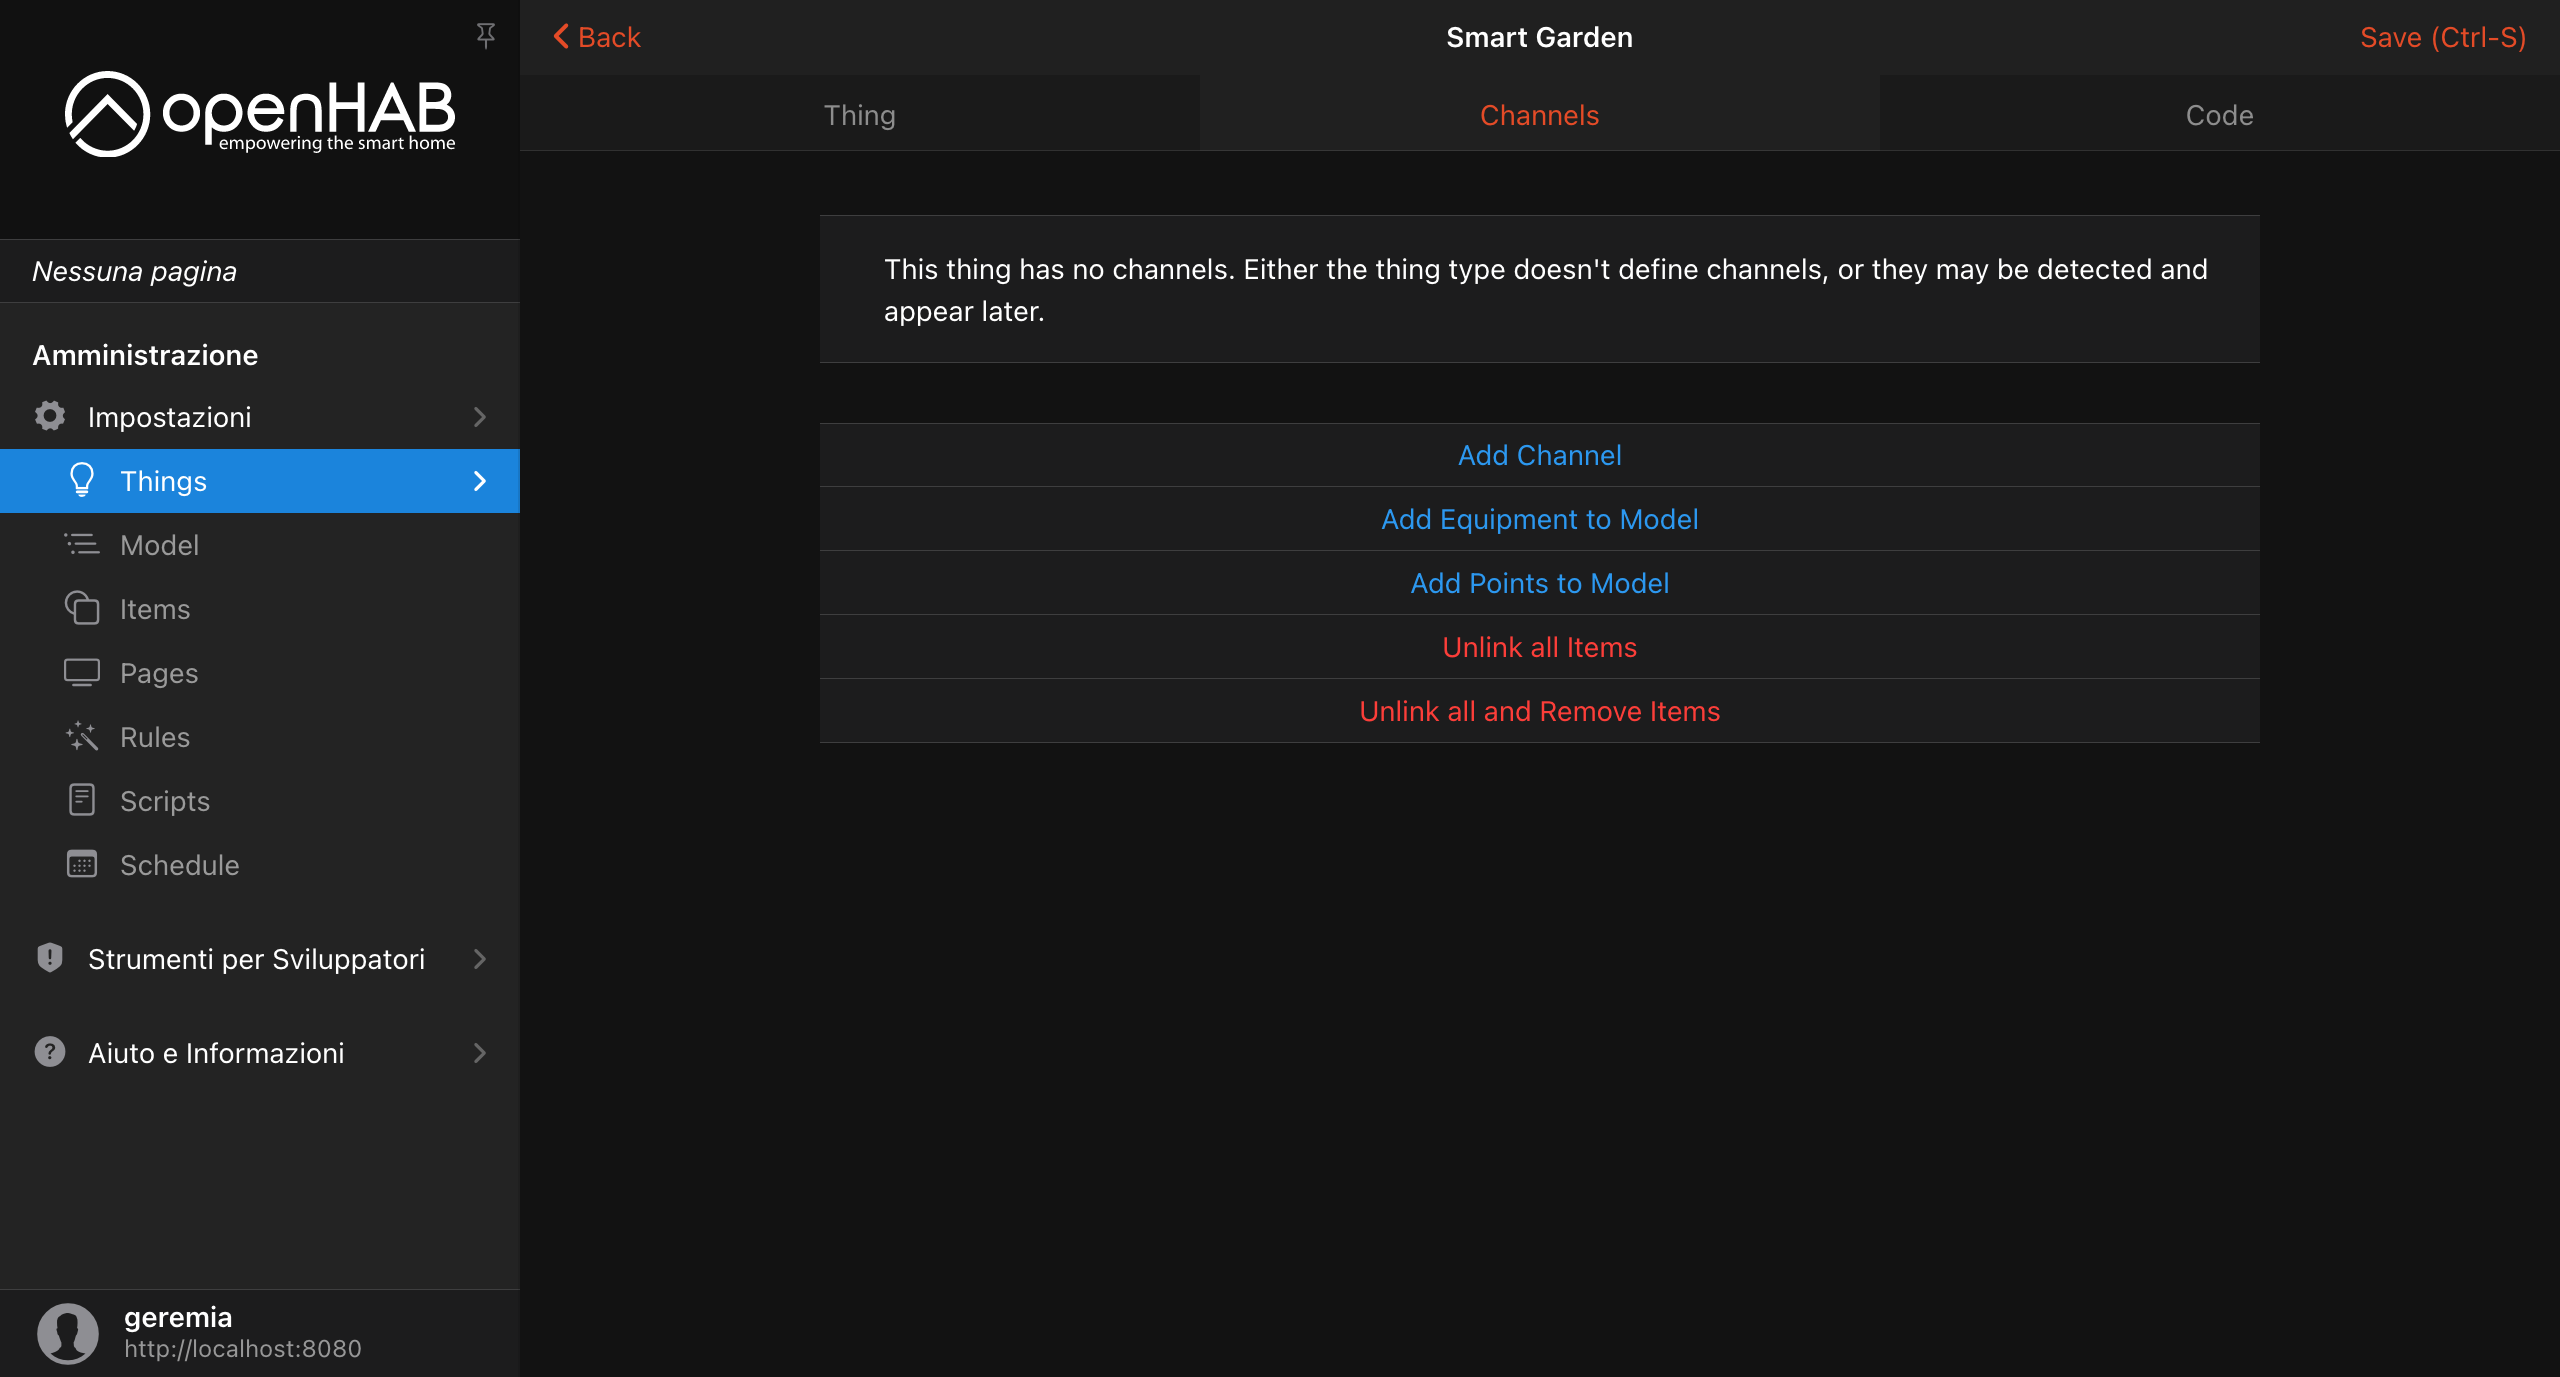
\includegraphics[width=12cm]{Immagini/channels}
        \caption{Schermata Channels}
        \label{fig:channels}
    \end{figure}
    \begin{figure}
        \centering
        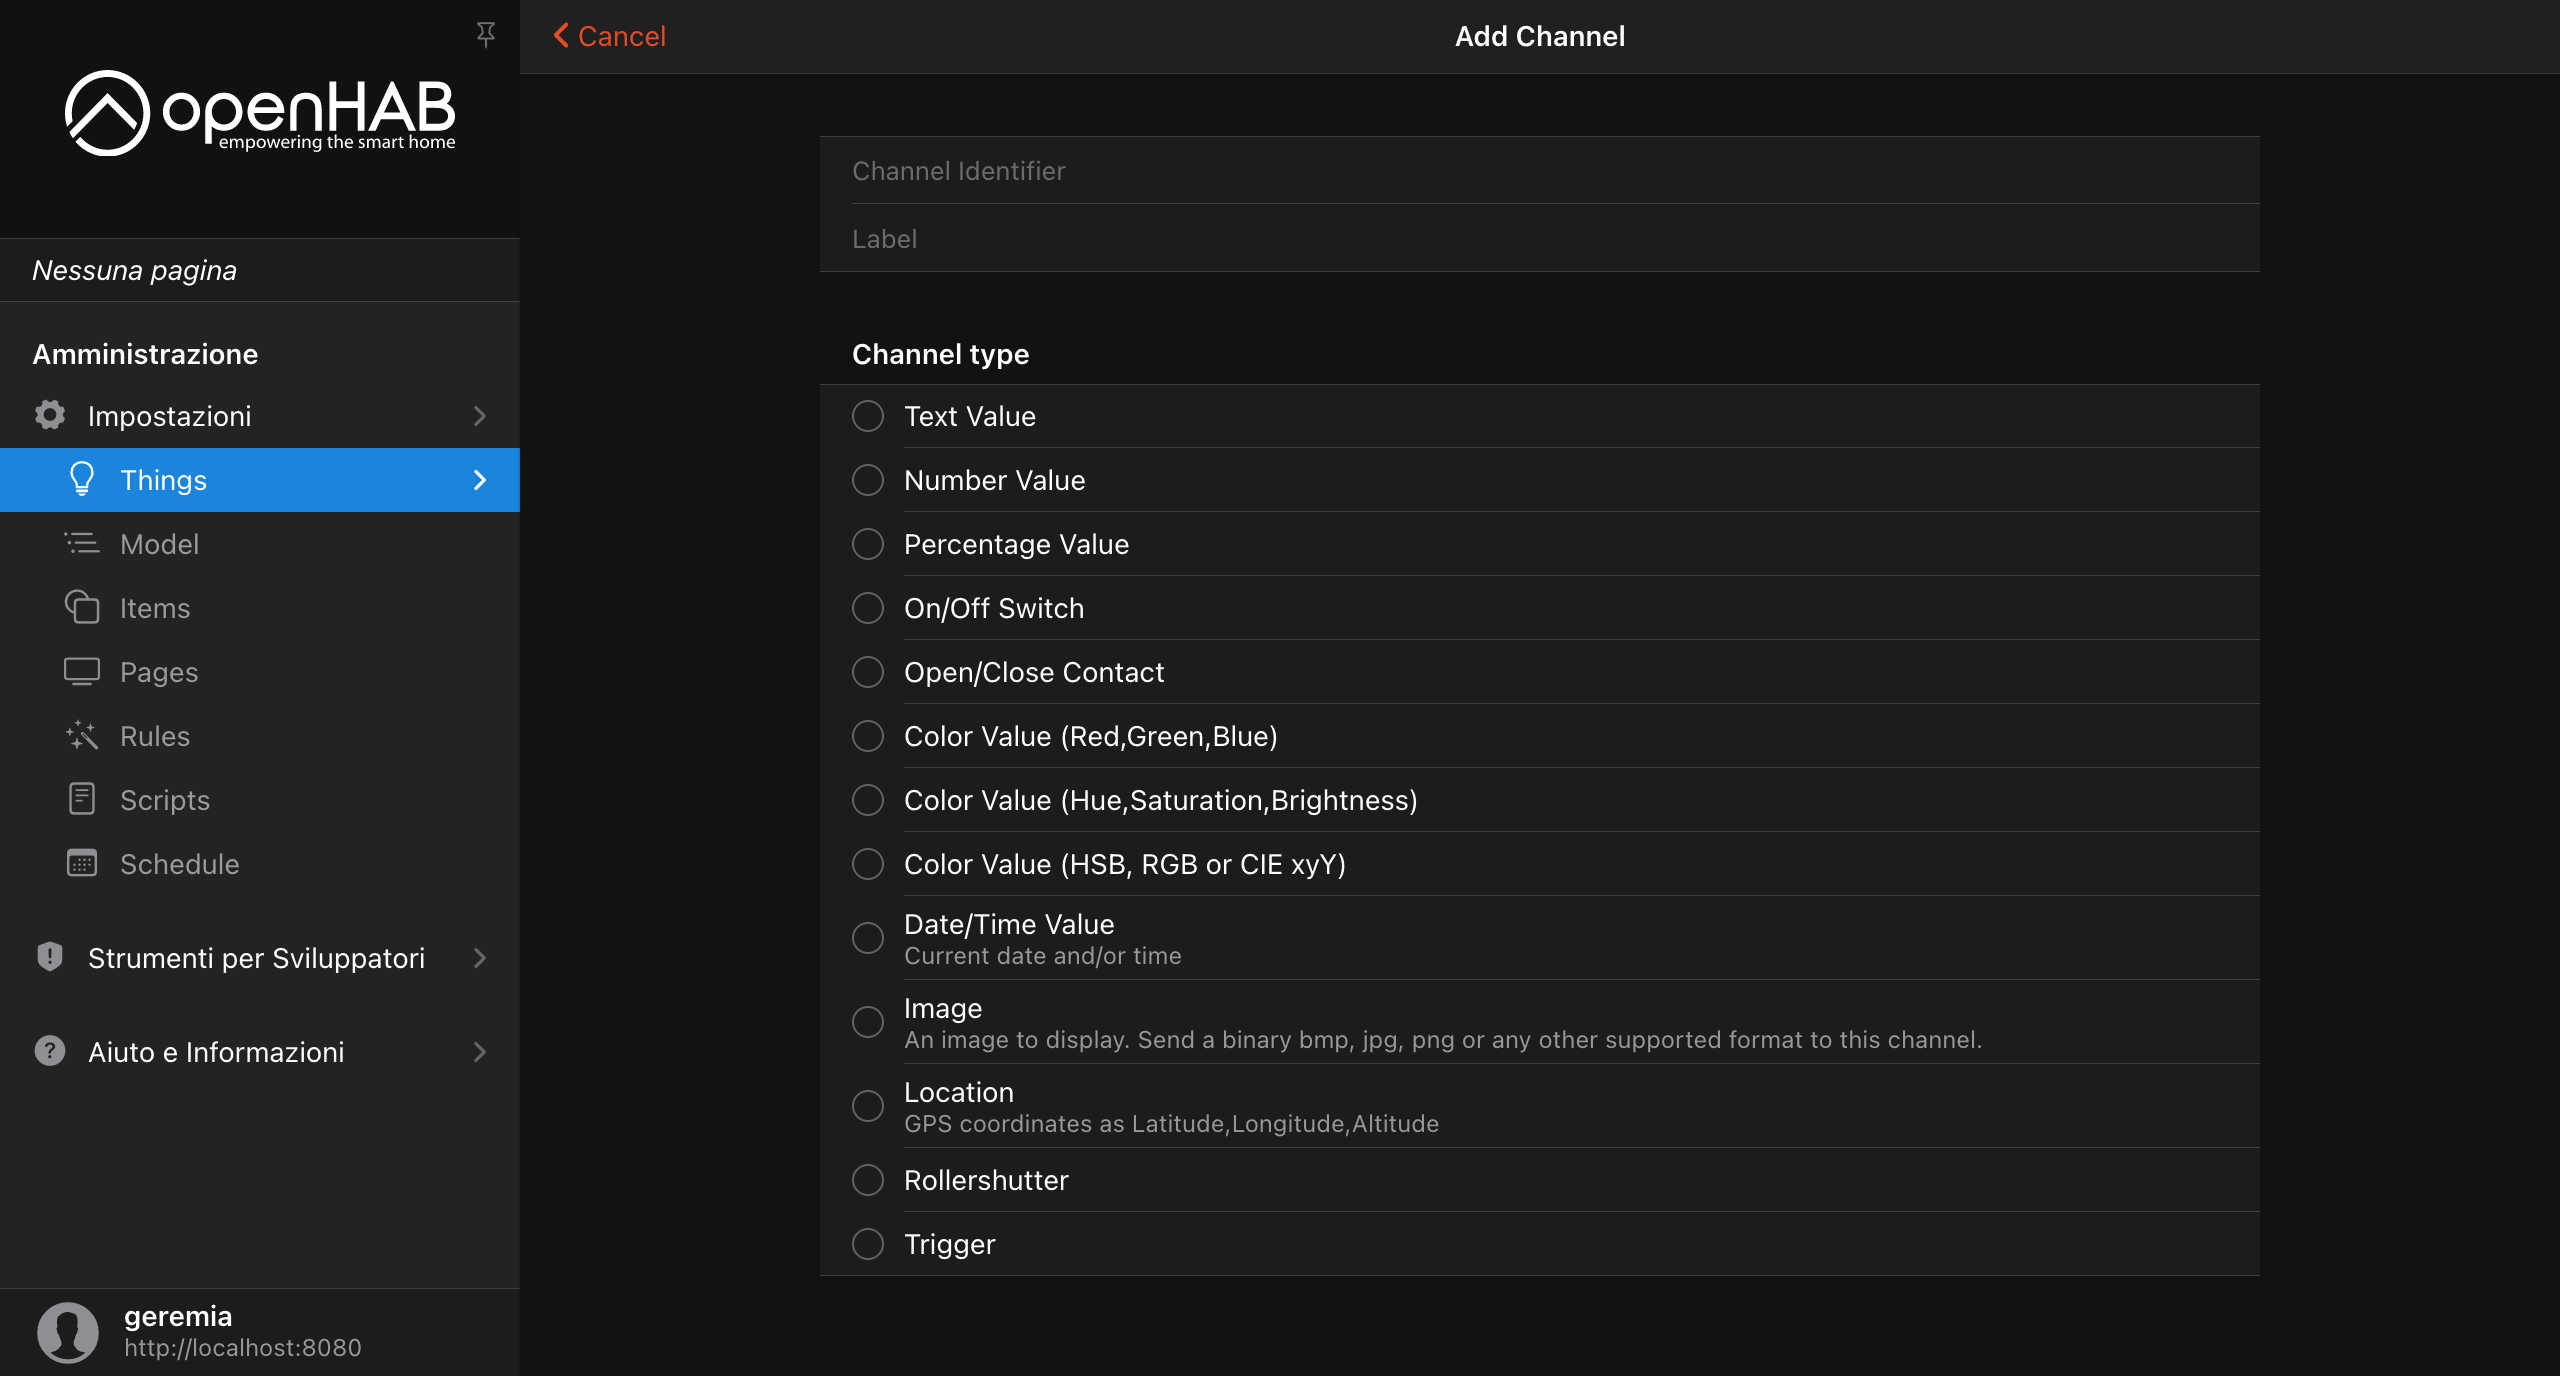
\includegraphics[width=12cm]{Immagini/add_channel}
        \caption{Schermata Add Channel}
        \label{fig:add_channel}
    \end{figure}
    \item successivamente per ogni channels dovrebbe essere creato un item. Per fare ci\'o basta selezionare il channel e premere ``Add Link to Item...''. Dalla schermata Channels quindi si passer\'a poi a quella ``Link Channel to Item'' in cui bisogna selezionare la voce ``Create new Item''. A questo punto basta selezionare una Category (in questo caso ``garden'') e premere ``Link''. Viene ripetuto tale procedimento per ogni Channel (Figura \ref{fig:link_channel_to_item})
    \begin{figure}
        \centering
        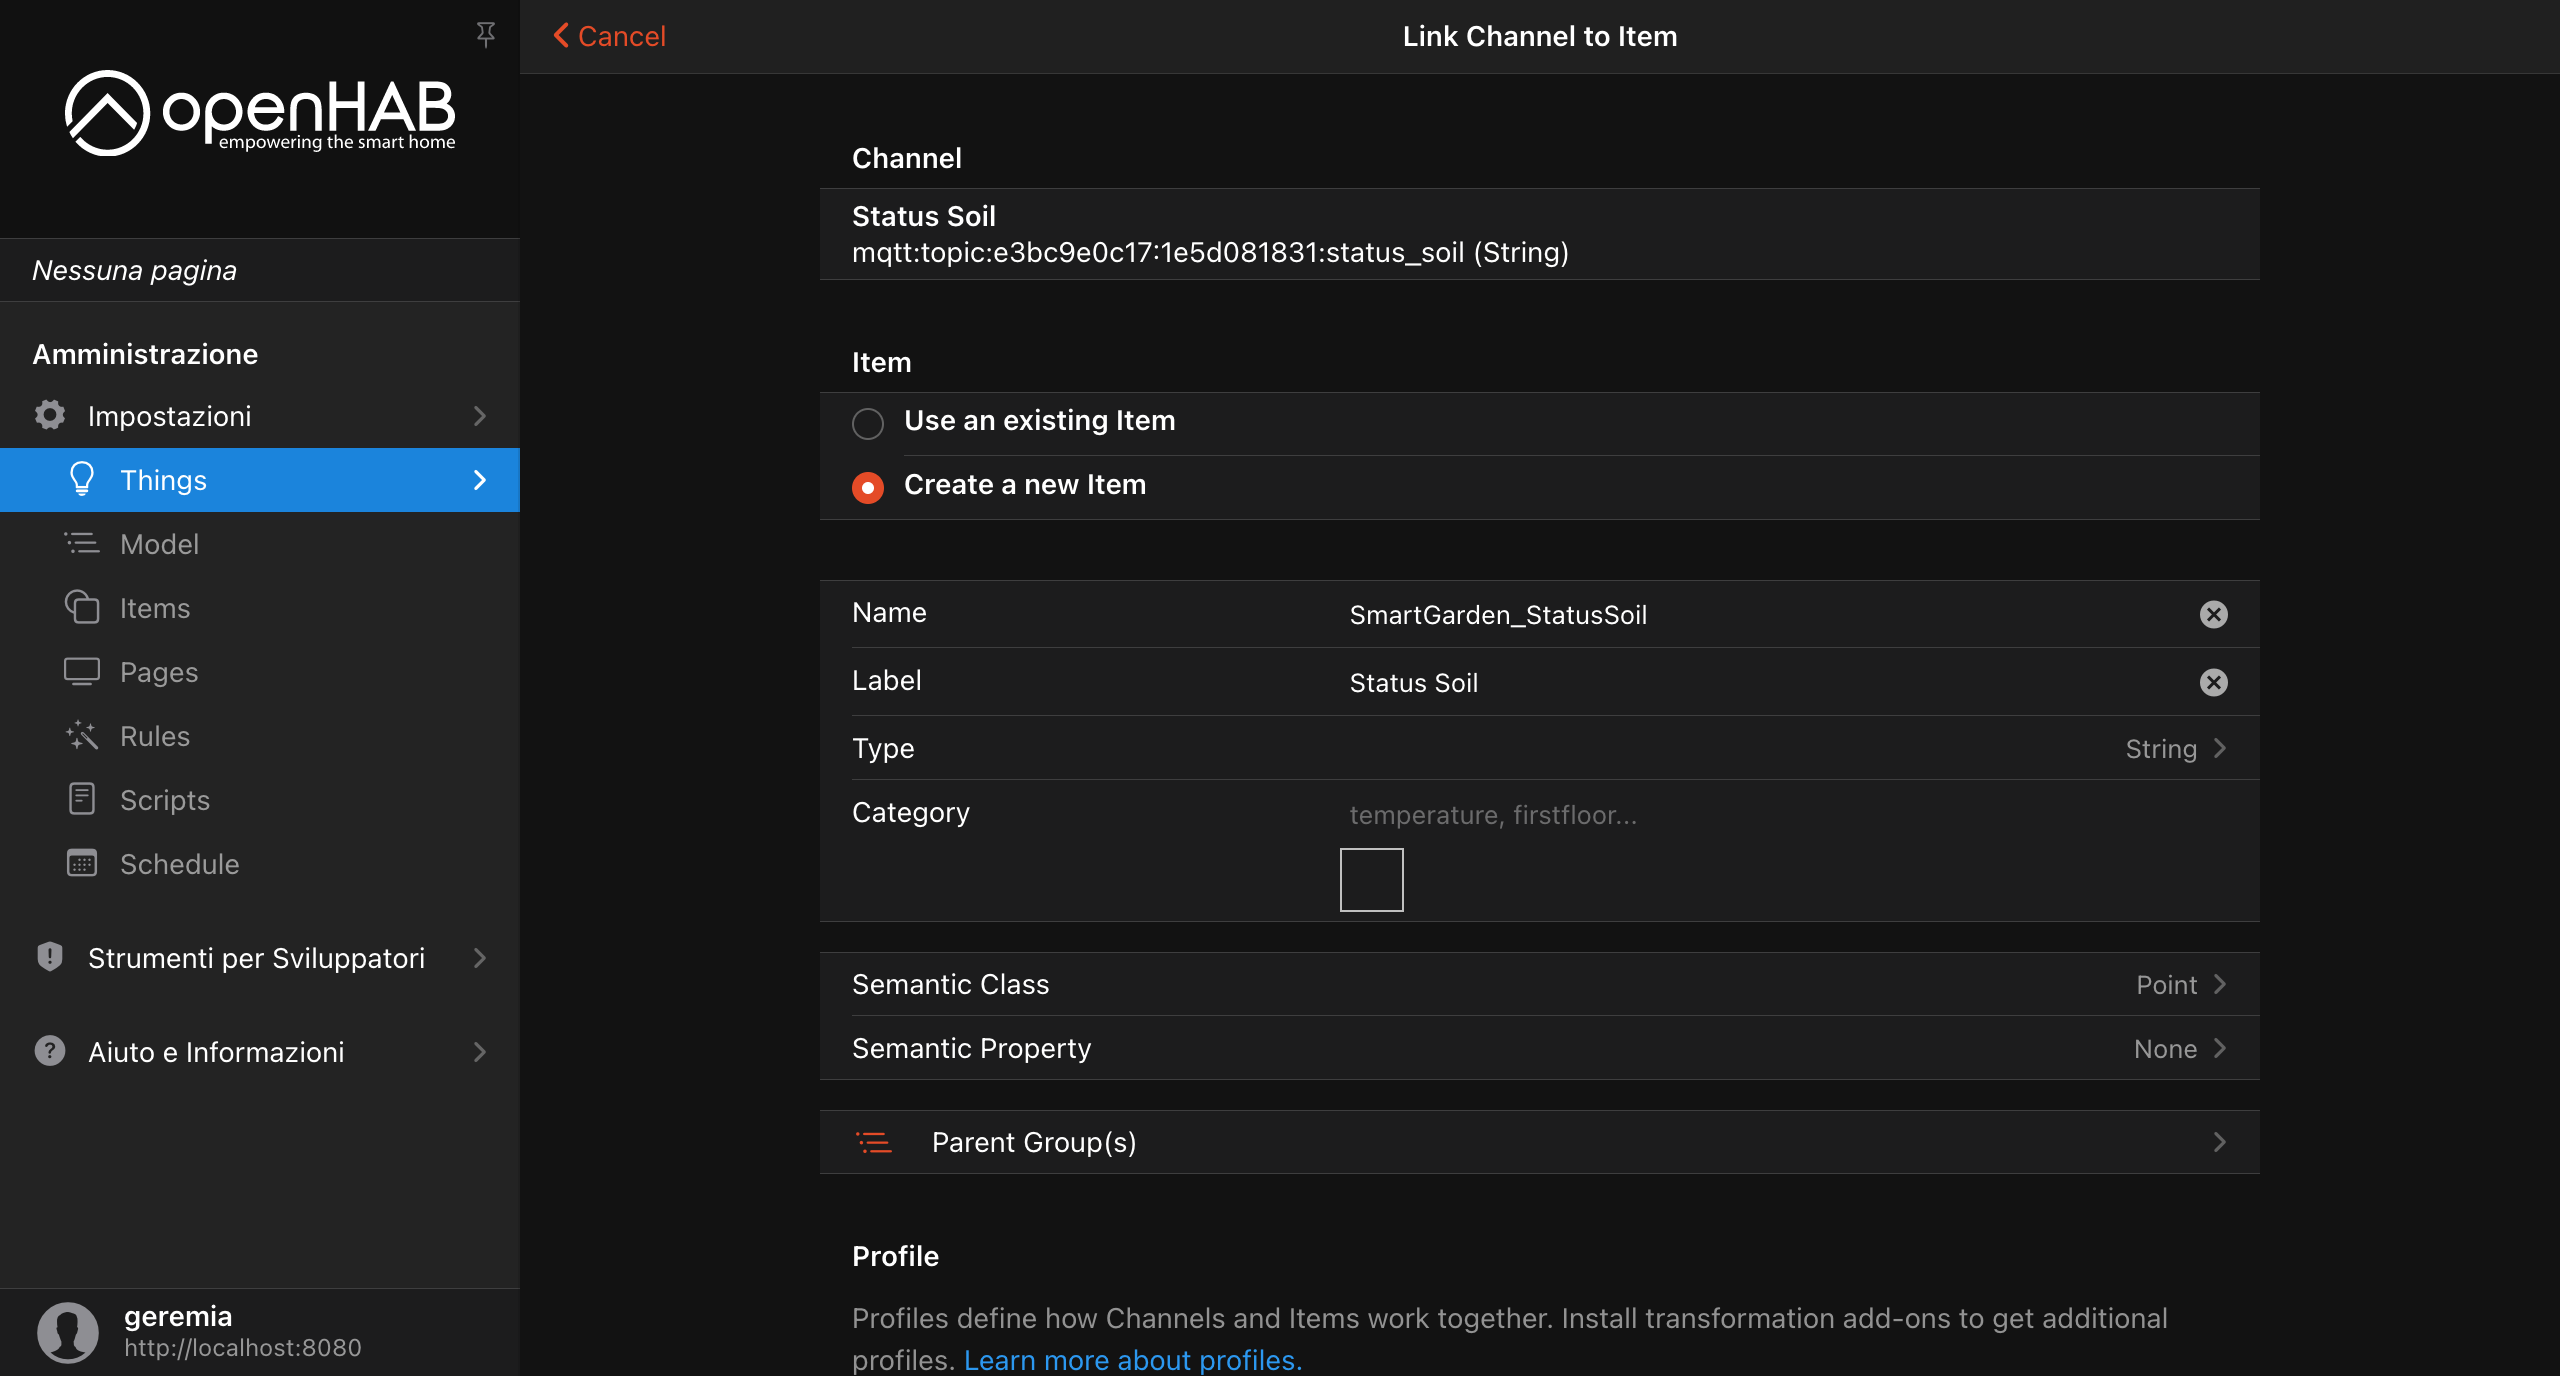
\includegraphics[width=12cm]{Immagini/link_channel_to_item}
        \caption{Schermata Link Channel to Item}
        \label{fig:link_channel_to_item}
    \end{figure}
\end{enumerate}
A questo punto se andiamo alla schermata Items sotto la voce Impostazioni del menu principale possiamo vedere gli Items gi\'a configurati (Figura \ref{fig:configured_items}). Se entriamo in uno di essi \'e possibile sia visualizzare lo stato che, in caso di items collegati a channels dinamici come lo Switch, eseguire un azione per cambiarlo.

\begin{figure}
    \centering
    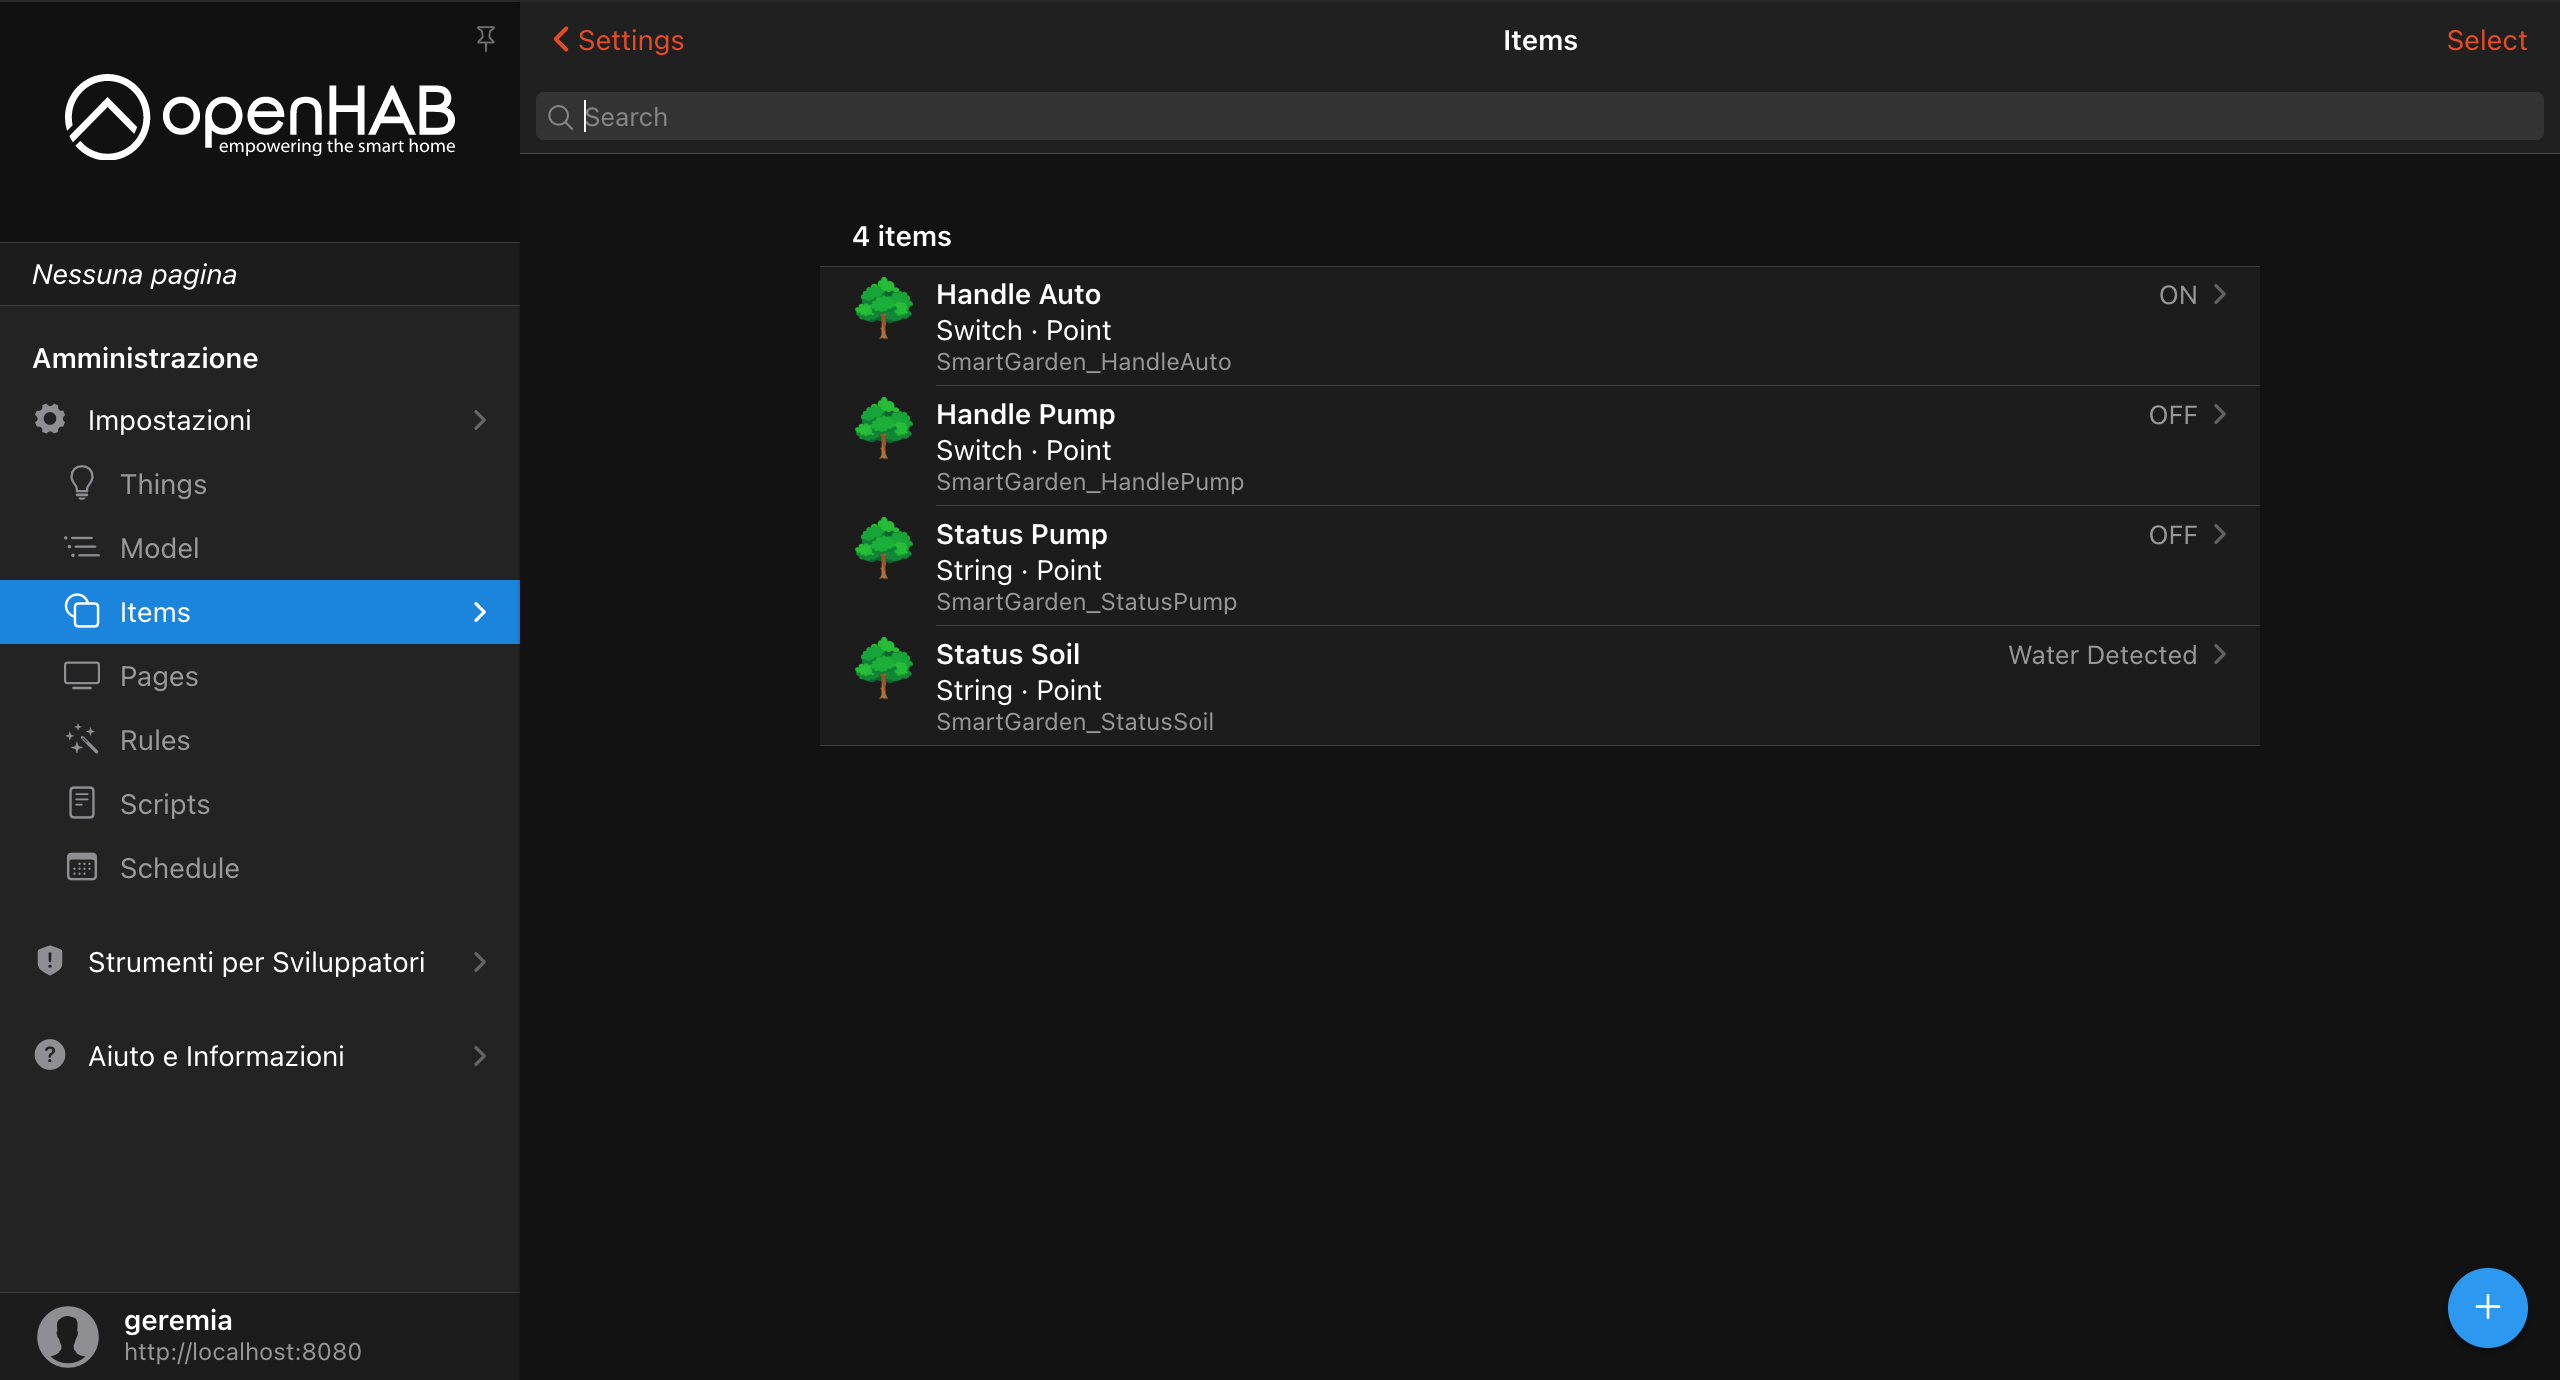
\includegraphics[width=12cm]{Immagini/configured_items}
    \caption{Items Configurati}
    \label{fig:configured_items}
\end{figure}

\subsection{Creazione Sitemap}
Per rendere il tutto pi\'u agevole e user friendly \'e possibile riportare tutto in una Sitemap. Per fare ci\'o bisogna agire all'interno della cartella ``config'' interna a sua volta alla folder principale del software openHAB. In questa cartella \'e possibile aggiungere i vari elementi di openHAB come items e things manualmente tramite file. A questo punto bisogna creare un file all'interno della cartella ``sitemaps'' nominato ``default.sitemap''. Questo \'e il file della Sitemap che andremo a creare. Il codice da scrivere all'interno sar\'a relativo agli Items aggiunti, infatti essi possono essere aggiunti tramite il loro identificativo che si trova nella propria schermata in alto. Possono essere aggiunte anche icone per rendere pi\'u immediata la schermata. In questo caso facciamo riferimento al Codice \ref{code:sitemap_smart_garden_code} dove troviamo il Frame ``Garden'' che contiene gli Items impostati precedentemente con relative icone e label (in caso di text value). \'E possibile poi visualizzare l'interfaccia web andando all'url \texttt{http://localhost:8080/basicui/app}. \'E possibile inoltre controllare ci\'o tramite smartphone installando l'applicazione di openHAB e configurandola aggiungendo indirizzo ip e porta del server openHAB interno alla propria rete locale (Figure \ref{fig:sitemap_smart_garden_ui_web} e \ref{fig:sitemap_smart_garden_ui_app}).

\begin{lstlisting}[caption=Sitemap Smart Garden Code,label=code:sitemap_smart_garden_code]
sitemap default label="Home"
{
    Frame label="Garden" 
    {
        Switch item=SmartGarden_HandlePump icon="switch"
        Switch item=SmartGarden_HandleAuto icon="switch"
        Text item=SmartGarden_StatusPump label="[%s]" icon="pump"
        Text item=SmartGarden_StatusSoil label="[%s]" icon="water"
    }
}
\end{lstlisting}

\begin{figure}
    \centering
    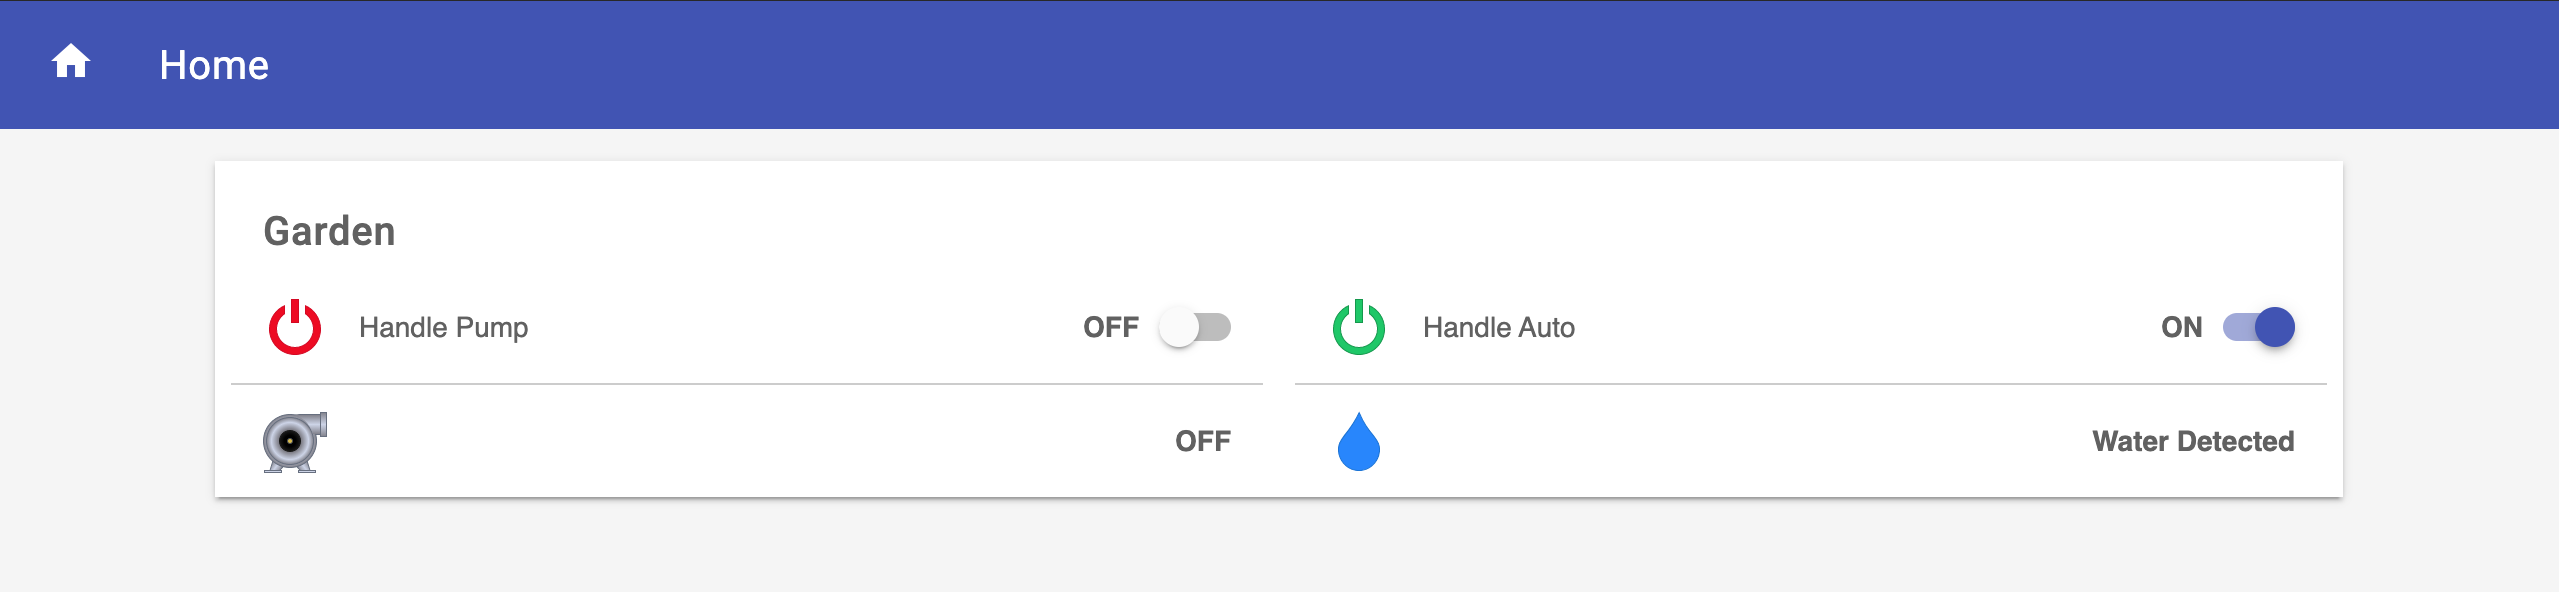
\includegraphics[width=12cm]{Immagini/sitemap_smart_garden_ui_web}
    \caption{Sitemap Smart Garden UI Web}
    \label{fig:sitemap_smart_garden_ui_web}
\end{figure}

\begin{figure}
    \centering
    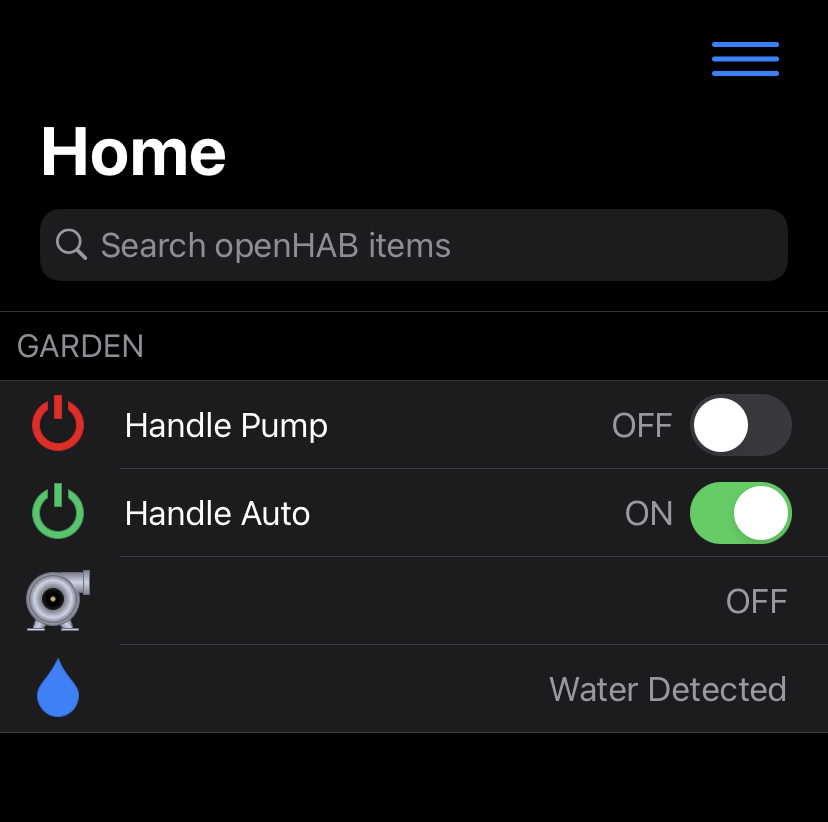
\includegraphics[width=12cm]{Immagini/sitemap_smart_garden_ui_app}
    \caption{Sitemap Smart Garden UI App}
    \label{fig:sitemap_smart_garden_ui_app}
\end{figure}